% Options for packages loaded elsewhere
\PassOptionsToPackage{unicode}{hyperref}
\PassOptionsToPackage{hyphens}{url}
\PassOptionsToPackage{dvipsnames,svgnames,x11names}{xcolor}
\documentclass[
  10pt,
]{extarticle}
\usepackage{xcolor}
\usepackage[top=1.5in, bottom=1.5in, left=1.5in, right=1.5in]{geometry}
\usepackage{amsmath,amssymb}
\setcounter{secnumdepth}{5}
\usepackage{iftex}
\ifPDFTeX
  \usepackage[T1]{fontenc}
  \usepackage[utf8]{inputenc}
  \usepackage{textcomp} % provide euro and other symbols
\else % if luatex or xetex
  \usepackage{unicode-math} % this also loads fontspec
  \defaultfontfeatures{Scale=MatchLowercase}
  \defaultfontfeatures[\rmfamily]{Ligatures=TeX,Scale=1}
\fi
\usepackage{lmodern}
\ifPDFTeX\else
  % xetex/luatex font selection
\fi
% Use upquote if available, for straight quotes in verbatim environments
\IfFileExists{upquote.sty}{\usepackage{upquote}}{}
\IfFileExists{microtype.sty}{% use microtype if available
  \usepackage[]{microtype}
  \UseMicrotypeSet[protrusion]{basicmath} % disable protrusion for tt fonts
}{}
\makeatletter
\@ifundefined{KOMAClassName}{% if non-KOMA class
  \IfFileExists{parskip.sty}{%
    \usepackage{parskip}
  }{% else
    \setlength{\parindent}{0pt}
    \setlength{\parskip}{6pt plus 2pt minus 1pt}}
}{% if KOMA class
  \KOMAoptions{parskip=half}}
\makeatother
\usepackage{color}
\usepackage{fancyvrb}
\newcommand{\VerbBar}{|}
\newcommand{\VERB}{\Verb[commandchars=\\\{\}]}
\DefineVerbatimEnvironment{Highlighting}{Verbatim}{commandchars=\\\{\}}
% Add ',fontsize=\small' for more characters per line
\usepackage{framed}
\definecolor{shadecolor}{RGB}{248,248,248}
\newenvironment{Shaded}{\begin{snugshade}}{\end{snugshade}}
\newcommand{\AlertTok}[1]{\textcolor[rgb]{0.94,0.16,0.16}{#1}}
\newcommand{\AnnotationTok}[1]{\textcolor[rgb]{0.56,0.35,0.01}{\textbf{\textit{#1}}}}
\newcommand{\AttributeTok}[1]{\textcolor[rgb]{0.13,0.29,0.53}{#1}}
\newcommand{\BaseNTok}[1]{\textcolor[rgb]{0.00,0.00,0.81}{#1}}
\newcommand{\BuiltInTok}[1]{#1}
\newcommand{\CharTok}[1]{\textcolor[rgb]{0.31,0.60,0.02}{#1}}
\newcommand{\CommentTok}[1]{\textcolor[rgb]{0.56,0.35,0.01}{\textit{#1}}}
\newcommand{\CommentVarTok}[1]{\textcolor[rgb]{0.56,0.35,0.01}{\textbf{\textit{#1}}}}
\newcommand{\ConstantTok}[1]{\textcolor[rgb]{0.56,0.35,0.01}{#1}}
\newcommand{\ControlFlowTok}[1]{\textcolor[rgb]{0.13,0.29,0.53}{\textbf{#1}}}
\newcommand{\DataTypeTok}[1]{\textcolor[rgb]{0.13,0.29,0.53}{#1}}
\newcommand{\DecValTok}[1]{\textcolor[rgb]{0.00,0.00,0.81}{#1}}
\newcommand{\DocumentationTok}[1]{\textcolor[rgb]{0.56,0.35,0.01}{\textbf{\textit{#1}}}}
\newcommand{\ErrorTok}[1]{\textcolor[rgb]{0.64,0.00,0.00}{\textbf{#1}}}
\newcommand{\ExtensionTok}[1]{#1}
\newcommand{\FloatTok}[1]{\textcolor[rgb]{0.00,0.00,0.81}{#1}}
\newcommand{\FunctionTok}[1]{\textcolor[rgb]{0.13,0.29,0.53}{\textbf{#1}}}
\newcommand{\ImportTok}[1]{#1}
\newcommand{\InformationTok}[1]{\textcolor[rgb]{0.56,0.35,0.01}{\textbf{\textit{#1}}}}
\newcommand{\KeywordTok}[1]{\textcolor[rgb]{0.13,0.29,0.53}{\textbf{#1}}}
\newcommand{\NormalTok}[1]{#1}
\newcommand{\OperatorTok}[1]{\textcolor[rgb]{0.81,0.36,0.00}{\textbf{#1}}}
\newcommand{\OtherTok}[1]{\textcolor[rgb]{0.56,0.35,0.01}{#1}}
\newcommand{\PreprocessorTok}[1]{\textcolor[rgb]{0.56,0.35,0.01}{\textit{#1}}}
\newcommand{\RegionMarkerTok}[1]{#1}
\newcommand{\SpecialCharTok}[1]{\textcolor[rgb]{0.81,0.36,0.00}{\textbf{#1}}}
\newcommand{\SpecialStringTok}[1]{\textcolor[rgb]{0.31,0.60,0.02}{#1}}
\newcommand{\StringTok}[1]{\textcolor[rgb]{0.31,0.60,0.02}{#1}}
\newcommand{\VariableTok}[1]{\textcolor[rgb]{0.00,0.00,0.00}{#1}}
\newcommand{\VerbatimStringTok}[1]{\textcolor[rgb]{0.31,0.60,0.02}{#1}}
\newcommand{\WarningTok}[1]{\textcolor[rgb]{0.56,0.35,0.01}{\textbf{\textit{#1}}}}
\usepackage{longtable,booktabs,array}
\newcounter{none} % for unnumbered tables
\usepackage{calc} % for calculating minipage widths
% Correct order of tables after \paragraph or \subparagraph
\usepackage{etoolbox}
\makeatletter
\patchcmd\longtable{\par}{\if@noskipsec\mbox{}\fi\par}{}{}
\makeatother
% Allow footnotes in longtable head/foot
\IfFileExists{footnotehyper.sty}{\usepackage{footnotehyper}}{\usepackage{footnote}}
\makesavenoteenv{longtable}
\usepackage{graphicx}
\makeatletter
\newsavebox\pandoc@box
\newcommand*\pandocbounded[1]{% scales image to fit in text height/width
  \sbox\pandoc@box{#1}%
  \Gscale@div\@tempa{\textheight}{\dimexpr\ht\pandoc@box+\dp\pandoc@box\relax}%
  \Gscale@div\@tempb{\linewidth}{\wd\pandoc@box}%
  \ifdim\@tempb\p@<\@tempa\p@\let\@tempa\@tempb\fi% select the smaller of both
  \ifdim\@tempa\p@<\p@\scalebox{\@tempa}{\usebox\pandoc@box}%
  \else\usebox{\pandoc@box}%
  \fi%
}
% Set default figure placement to htbp
\def\fps@figure{htbp}
\makeatother
\setlength{\emergencystretch}{3em} % prevent overfull lines
\providecommand{\tightlist}{%
  \setlength{\itemsep}{0pt}\setlength{\parskip}{0pt}}
\usepackage{xcolor}
\usepackage{hyperref}
\hypersetup{colorlinks=true, linkcolor=blue, urlcolor=blue, citecolor=blue}
\usepackage{float}
\usepackage{fvextra}
\usepackage{fancyhdr}
\usepackage{lastpage}
\usepackage{soul}
\usepackage{etoolbox}
\usepackage{microtype}
\usepackage{tcolorbox}
\usepackage{enumitem}
\usepackage{fancyvrb}
\usepackage{xspace}
\allowdisplaybreaks
\setcounter{tocdepth}{2}
\setcounter{secnumdepth}{0}
\floatplacement{figure}{H}
\makeatletter
\newcommand{\@subtitle}{}
\newcommand{\subtitle}[1]{\gdef\@subtitle{#1}}
\newcommand{\DocSubtitle}{\@subtitle}
\renewcommand{\maketitle}{
  \thispagestyle{plain}
  \null
  \vfill
  \begin{center}
    {\Large \textsc{\@title} \par}\vskip 0.5em
    {\LARGE \bfseries \@subtitle \par}\vskip 0.75em
    {\large \@author \par}\vskip 0.5em
    {\normalsize \@date \par}
  \end{center}
  \vfill
  \tableofcontents
  \vspace{1em}
  \clearpage
}
\AfterEndEnvironment{Highlighting}{\setcounter{CodeLine}{\numexpr\value{CodeLine}+\FV@CodeLineNo\relax}}
\makeatother
\fancypagestyle{plain}{
  \fancyhf{}
  \renewcommand{\headrulewidth}{0pt}
  \renewcommand{\footrulewidth}{0pt}
}
\pagestyle{fancy}
\fancyhf{}
\fancyfoot[C]{\small\textsc{Page}~\thepage~\textsc{of}~\pageref{LastPage}}
\fancyhead[L]{\textsc{Rento Saijo}}
\fancyhead[R]{\textsc{\DocSubtitle}}
\fancyhead[C]{\textsc{\rightmark}}
\renewcommand{\headrulewidth}{0.5pt}
\renewcommand{\footrulewidth}{0.5pt}
\newcounter{CodeLine}
\newcounter{cell}
\AtBeginEnvironment{Highlighting}{\stepcounter{cell}}
\DefineVerbatimEnvironment{Highlighting}{Verbatim}{
  frame=single,
  rulecolor=\color{black},
  framesep=2mm,
  label=\footnotesize Cell \thecell,
  labelposition=topline,
  commandchars=\\\{\},
  breaklines=true,
  breakanywhere=false,
  breaksymbol={},
  numbers=left,
  numbersep=3pt,
  firstnumber=\numexpr\value{CodeLine}+1\relax,
  fontsize=\small
}
\DefineVerbatimEnvironment{verbatim}{Verbatim}{
  breaklines=true,
  breakanywhere=true,
  numbers=left,
  numbersep=3pt,
  firstnumber=1,
  fontsize=\footnotesize
}
\newtcolorbox{problem}[1][]{
  title={\textsc{#1}}
}
\renewcommand{\contentsname}{Table of Contents}
\newcommand{\E}{\mathrm{E}}
\newcommand{\Var}{\mathrm{Var}}
\newcommand{\Cov}{\mathrm{Cov}}
\newcommand{\R}{\textsf{R}\xspace}
\newcommand{\SD}{\mathrm{SD}}
\newcommand{\SE}{\mathrm{SE}}
\usepackage{bookmark}
\IfFileExists{xurl.sty}{\usepackage{xurl}}{} % add URL line breaks if available
\urlstyle{same}
\hypersetup{
  pdftitle={STA 209: Introduction to Time Series Analysis},
  colorlinks=true,
  linkcolor={blue},
  filecolor={Maroon},
  citecolor={blue},
  urlcolor={blue},
  pdfcreator={LaTeX via pandoc}}

\title{STA 209: Introduction to Time Series Analysis}
\usepackage{etoolbox}
\makeatletter
\providecommand{\subtitle}[1]{% add subtitle to \maketitle
  \apptocmd{\@title}{\par {\large #1 \par}}{}{}
}
\makeatother
\subtitle{Homework 7}
\author{Rento Saijo}
\date{May 1, 2026}

\begin{document}
\maketitle

\section{Disclosure}\label{disclosure}

GPT-5.4 (High) on Codex was used to create the \texttt{YAML} portion and some \texttt{LaTeX} code to format the text and equations. Page-formatting code was also provided by Derin Gezgin. In the setup, chunk options were set for the document, and helper functions were defined for repetitive plotting, table-formatting, CCF, regression, transformation, and ARMA/ARIMA fitting steps. See the original \texttt{RMD} file \href{https://github.com/RentoSaijo/STA209/blob/main/Homework7.Rmd}{here} for more details.

\newpage

\section{Problem 1}\label{problem-1}

\begin{problem}[Problem 1]
Answer the following questions for your data project.
\end{problem}

\newpage

\subsection{Problem 1 (a)}\label{problem-1-a}

\begin{problem}[Problem 1 (a)]
Briefly introduce the problem you are exploring and briefly state the variables you are using.
\end{problem}

My project studies whether a hockey goalie's even-strength goals saved above expected, or GSAx, is really as team-independent as it is often interpreted to be. The comparison uses Mackenzie Blackwood and Igor Shesterkin because Blackwood's team context changed substantially across New Jersey, San Jose, and Colorado, while Shesterkin remained with the New York Rangers in the matched sample. This makes the project a time-series comparison of one goalie with major team-context changes and one goalie with much more organizational continuity. I use the game-by-game even-strength variables
\[
\begin{aligned}
G_t &= \text{game-by-game even-strength GSAx},\\
S_t &= \text{game-by-game even-strength save percentage},\\
X_t &= \text{team even-strength xGF\%}.
\end{aligned}
\]
Here, \(G_t\) is measured in goals, \(S_t\) is recorded as a proportion, and \(X_t\) is measured in percentage points. The response variable is \(G_t\). The predictors are \(S_t\) and \(X_t\). The time variable \(t\) is the matched career game number. For each goalie, the frequency is one observation per completed regular-season game, so the series has frequency \(1\) in \textsf{R}. The range is \(t = 1,2,\ldots,285\). For Blackwood, this covers 2018-12-18 through 2026-03-28, with 152 games for New Jersey, 63 games for San Jose, and 70 games for Colorado. For Shesterkin, this covers 2020-01-07 through 2025-11-04, and all 285 games are with the Rangers.

\newpage

\subsection{Problem 1 (b)}\label{problem-1-b}

\begin{problem}[Problem 1 (b)]
Are the variables (time series) in your data stationary? Justify using the time-series plots and ADF tests.
\end{problem}

\subsubsection{Blackwood}\label{blackwood}

\begin{Shaded}
\begin{Highlighting}[]
\FunctionTok{with\_family}\NormalTok{(\{}
  \FunctionTok{plot\_raw\_series}\NormalTok{(blackwood\_gbgs, }\StringTok{\textquotesingle{}Blackwood\textquotesingle{}}\NormalTok{, }\AttributeTok{add\_trade\_lines =} \ConstantTok{TRUE}\NormalTok{)}
\NormalTok{\})}
\end{Highlighting}
\end{Shaded}

\begin{center}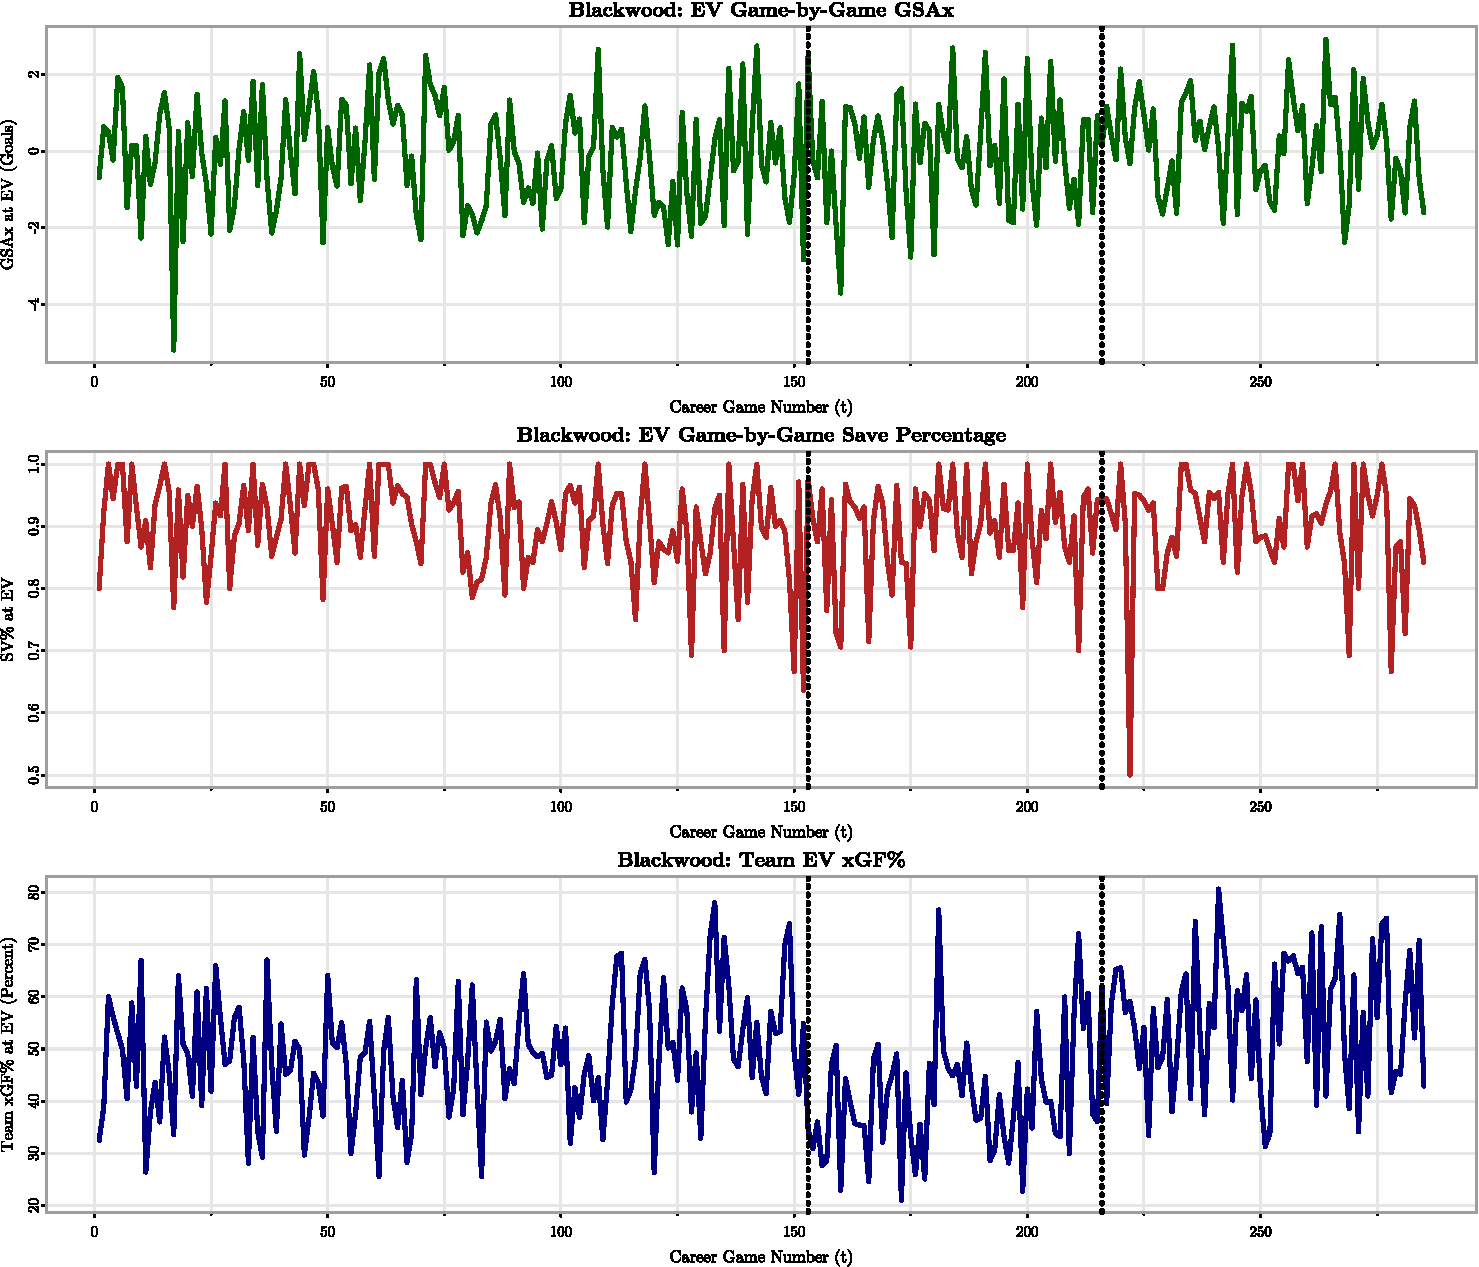
\includegraphics[width=\linewidth]{Homework7_files/figure-latex/p1-raw-plots-blackwood-1} \end{center}

\begin{itemize}
\tightlist
\item
  \(G_t\): This is Blackwood's game-by-game even-strength GSAx series, measured in goals, over 285 matched career games from 2018-12-18 through 2026-03-28. The plot does not show a sustained linear or nonlinear trend. Instead, it oscillates around a roughly stable center near -0.04 goals, with isolated positive and negative spikes. There is no repeated seasonal pattern in the game index. The variability looks fairly stable over time, so there is no strong visual evidence of heteroscedasticity, although individual games can be extreme. There is no clear volatility clustering. The statistical range is -5.1899 to 2.9214, so the total range is 8.1113 goals.
\item
  \(S_t\): This is Blackwood's game-by-game even-strength save percentage series, measured as a proportion. The mean behavior appears approximately stable around 0.9023, with no clear linear or nonlinear trend through the matched game index. There is no visible seasonal pattern. The series has a few sharp downward games, but these appear as isolated dips rather than a repeating cycle. The spread appears reasonably constant over time, so the variance looks approximately homoscedastic. There is no clear volatility clustering. The statistical range is 0.5 to 1, so the total range is 0.5.
\item
  \(X_t\): This is Blackwood's team game-by-game even-strength xGF\% series, measured in percentage points. The plot fluctuates around 48.59 percent. Franchise changes create local level differences, but the overall movement is still irregular rather than a sustained deterministic trend. There is no visual seasonality. The variance looks approximately constant over time, although there are isolated team-context outliers. There is no clear volatility clustering. The statistical range is 21.03 to 80.66, so the total range is 59.63 percentage points.
\end{itemize}

Overall, the Blackwood series look approximately stationary from the time-series plots. The means appear stable enough for the game-by-game analysis, and the spreads do not show persistent fanning-in or fanning-out.

\subsubsection{Shesterkin}\label{shesterkin}

\begin{Shaded}
\begin{Highlighting}[]
\FunctionTok{with\_family}\NormalTok{(\{}
  \FunctionTok{plot\_raw\_series}\NormalTok{(shesterkin\_gbgs, }\StringTok{\textquotesingle{}Shesterkin\textquotesingle{}}\NormalTok{, }\AttributeTok{add\_trade\_lines =} \ConstantTok{FALSE}\NormalTok{)}
\NormalTok{\})}
\end{Highlighting}
\end{Shaded}

\begin{center}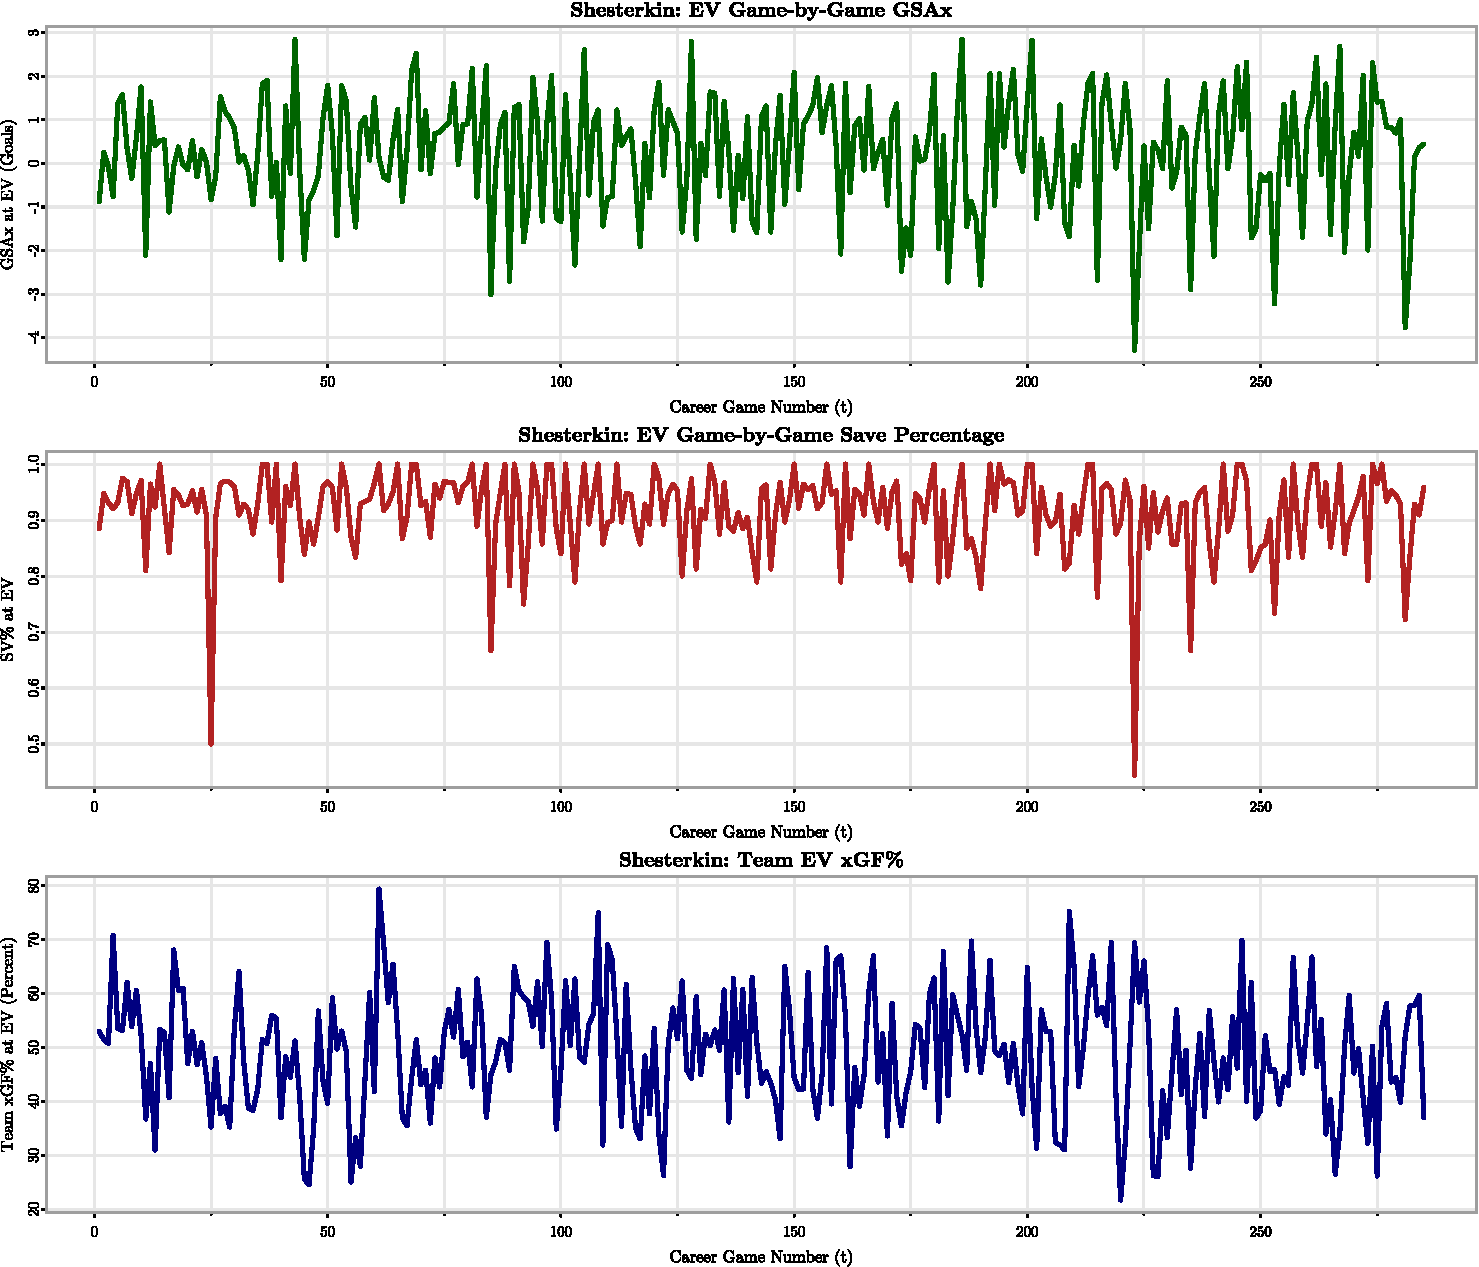
\includegraphics[width=\linewidth]{Homework7_files/figure-latex/p1-raw-plots-shesterkin-1} \end{center}

\begin{itemize}
\tightlist
\item
  \(G_t\): This is Shesterkin's game-by-game even-strength GSAx series, measured in goals, over 285 matched career games from 2020-01-07 through 2025-11-04. The plot fluctuates around a stable positive center near 0.2329 goals and does not show a visible linear or nonlinear trend. There is no visible seasonal cycle. The spikes are irregular rather than repeating. The spread appears fairly stable over time, so the variance looks approximately homoscedastic, although the later part has somewhat wider individual games. There is no clear volatility clustering. The statistical range is -4.288 to 2.857, so the total range is 7.1451 goals.
\item
  \(S_t\): This is Shesterkin's game-by-game even-strength save percentage series, measured as a proportion. The series fluctuates around 0.9163, with occasional large downward games, but it does not show a systematic linear or nonlinear trend. There is no clear repeated seasonal pattern. The variance is fairly stable, with a few isolated low-save-percentage games rather than a persistent fanning pattern. There is no clear volatility clustering. The statistical range is 0.4444 to 1, so the total range is 0.5556.
\item
  \(X_t\): This is Shesterkin's team game-by-game even-strength xGF\% series, measured in percentage points. The plot oscillates around 49.07 percent, and the movement appears irregular rather than trending. There is no visible seasonal pattern. The spread looks fairly stable over time, so there is no strong visual evidence of heteroscedasticity or volatility clustering. The statistical range is 21.68 to 79.42, so the total range is 57.74 percentage points.
\end{itemize}

Overall, the Shesterkin series also appear approximately stationary from the time-series plots. The means look stable, and the variances are reasonably constant. For a formal check, I use the Augmented Dickey-Fuller test. The null hypothesis is
\[
H_0: \text{the series is non-stationary},
\]
and the alternative is
\[
H_a: \text{the series is stationary}.
\]

\begin{Shaded}
\begin{Highlighting}[]
\NormalTok{tseries}\SpecialCharTok{::}\FunctionTok{adf.test}\NormalTok{(blackwood\_gbgs}\SpecialCharTok{$}\NormalTok{gsax\_ev)}
\end{Highlighting}
\end{Shaded}

\begin{verbatim}
## 
##  Augmented Dickey-Fuller Test
## 
## data:  blackwood_gbgs$gsax_ev
## Dickey-Fuller = -6.7931, Lag order = 6, p-value = 0.01
## alternative hypothesis: stationary
\end{verbatim}

\begin{Shaded}
\begin{Highlighting}[]
\NormalTok{tseries}\SpecialCharTok{::}\FunctionTok{adf.test}\NormalTok{(blackwood\_gbgs}\SpecialCharTok{$}\NormalTok{sv\_pct\_ev)}
\end{Highlighting}
\end{Shaded}

\begin{verbatim}
## 
##  Augmented Dickey-Fuller Test
## 
## data:  blackwood_gbgs$sv_pct_ev
## Dickey-Fuller = -6.0001, Lag order = 6, p-value = 0.01
## alternative hypothesis: stationary
\end{verbatim}

\begin{Shaded}
\begin{Highlighting}[]
\NormalTok{tseries}\SpecialCharTok{::}\FunctionTok{adf.test}\NormalTok{(blackwood\_gbgs}\SpecialCharTok{$}\NormalTok{team\_xg\_pct\_ev)}
\end{Highlighting}
\end{Shaded}

\begin{verbatim}
## 
##  Augmented Dickey-Fuller Test
## 
## data:  blackwood_gbgs$team_xg_pct_ev
## Dickey-Fuller = -4.1809, Lag order = 6, p-value = 0.01
## alternative hypothesis: stationary
\end{verbatim}

\begin{Shaded}
\begin{Highlighting}[]
\NormalTok{tseries}\SpecialCharTok{::}\FunctionTok{adf.test}\NormalTok{(shesterkin\_gbgs}\SpecialCharTok{$}\NormalTok{gsax\_ev)}
\end{Highlighting}
\end{Shaded}

\begin{verbatim}
## 
##  Augmented Dickey-Fuller Test
## 
## data:  shesterkin_gbgs$gsax_ev
## Dickey-Fuller = -6.7433, Lag order = 6, p-value = 0.01
## alternative hypothesis: stationary
\end{verbatim}

\begin{Shaded}
\begin{Highlighting}[]
\NormalTok{tseries}\SpecialCharTok{::}\FunctionTok{adf.test}\NormalTok{(shesterkin\_gbgs}\SpecialCharTok{$}\NormalTok{sv\_pct\_ev)}
\end{Highlighting}
\end{Shaded}

\begin{verbatim}
## 
##  Augmented Dickey-Fuller Test
## 
## data:  shesterkin_gbgs$sv_pct_ev
## Dickey-Fuller = -6.9665, Lag order = 6, p-value = 0.01
## alternative hypothesis: stationary
\end{verbatim}

\begin{Shaded}
\begin{Highlighting}[]
\NormalTok{tseries}\SpecialCharTok{::}\FunctionTok{adf.test}\NormalTok{(shesterkin\_gbgs}\SpecialCharTok{$}\NormalTok{team\_xg\_pct\_ev)}
\end{Highlighting}
\end{Shaded}

\begin{verbatim}
## 
##  Augmented Dickey-Fuller Test
## 
## data:  shesterkin_gbgs$team_xg_pct_ev
## Dickey-Fuller = -6.8293, Lag order = 6, p-value = 0.01
## alternative hypothesis: stationary
\end{verbatim}

\begin{center}
\scriptsize
\begin{table}[H]

\caption{\label{tab:p1-adf-table}ADF test results for the project time series}
\centering
\begin{tabular}[t]{cccccc}
\toprule
Goalie & Series & DF & Lag & P-value & Decision\\
\midrule
Blackwood & $G_t$ & -6.7931 & 6 & <0.01 & Reject $H_0$\\
Blackwood & $S_t$ & -6.0001 & 6 & <0.01 & Reject $H_0$\\
Blackwood & $X_t$ & -4.1809 & 6 & <0.01 & Reject $H_0$\\
Shesterkin & $G_t$ & -6.7433 & 6 & <0.01 & Reject $H_0$\\
Shesterkin & $S_t$ & -6.9665 & 6 & <0.01 & Reject $H_0$\\
\addlinespace
Shesterkin & $X_t$ & -6.8293 & 6 & <0.01 & Reject $H_0$\\
\bottomrule
\end{tabular}
\end{table}
\normalsize
\end{center}

All six ADF tests reject \(H_0\) at the 5\% level. Therefore, the ADF results support the visual conclusion that the response and predictor series are stationary enough for the constant-level trend model and the later time-series regression step.

\newpage

\subsection{Problem 1 (c)}\label{problem-1-c}

\begin{problem}[Problem 1 (c)]
If there is any trend in your data, model the average overall trend using techniques learned in class.
\end{problem}

Since the raw game-by-game response and predictors appear stationary, I do not fit nonconstant polynomial trend models for these six series (i.e., for trend modeling, the appropriate conclusion is that the nonconstant trend terms are unnecessary). A descriptive constant-level model is
\[
Y_t = \mu_Y + W_t,
\]
where \(Y_t\) is one of \(G_t\), \(S_t\), or \(X_t\), and \(W_t\) is the remaining noise. For Blackwood, the fitted mean models are
\[
\begin{aligned}
G_t &= -0.039974 + W_t,\\
S_t &= 0.902272 + W_t,\\
X_t &= 48.591400 + W_t.
\end{aligned}
\]
For Shesterkin, the fitted mean models are
\[
\begin{aligned}
G_t &= 0.232914 + W_t,\\
S_t &= 0.916254 + W_t,\\
X_t &= 49.065530 + W_t.
\end{aligned}
\]
In these equations, \(t\) is the career-game index \(1,\ldots,285\).
For the remaining modeling steps, I remove these fitted average levels and work with the detrended variables
\[
\tilde{G}_t = G_t - \hat{\mu}_G,\qquad
\tilde{S}_t = S_t - \hat{\mu}_S,\qquad
\tilde{X}_t = X_t - \hat{\mu}_X.
\]
These are still measured in the same units as the original series: \(\tilde{G}_t\) is in goals, \(\tilde{S}_t\) is in save-percentage proportion units, and \(\tilde{X}_t\) is in percentage points. The only change is that each series is now measured as a deviation from its fitted average level.

\newpage

\subsection{Problem 1 (d)}\label{problem-1-d}

\begin{problem}[Problem 1 (d)]
Is there any seasonality? Determine using the periodogram and state what is the periodicity.
\end{problem}

\begin{Shaded}
\begin{Highlighting}[]
\FunctionTok{with\_family}\NormalTok{(\{}
  \FunctionTok{plot\_periodograms}\NormalTok{(blackwood\_detrended, }\StringTok{\textquotesingle{}Blackwood Detrended\textquotesingle{}}\NormalTok{)}
\NormalTok{\})}
\end{Highlighting}
\end{Shaded}

\begin{center}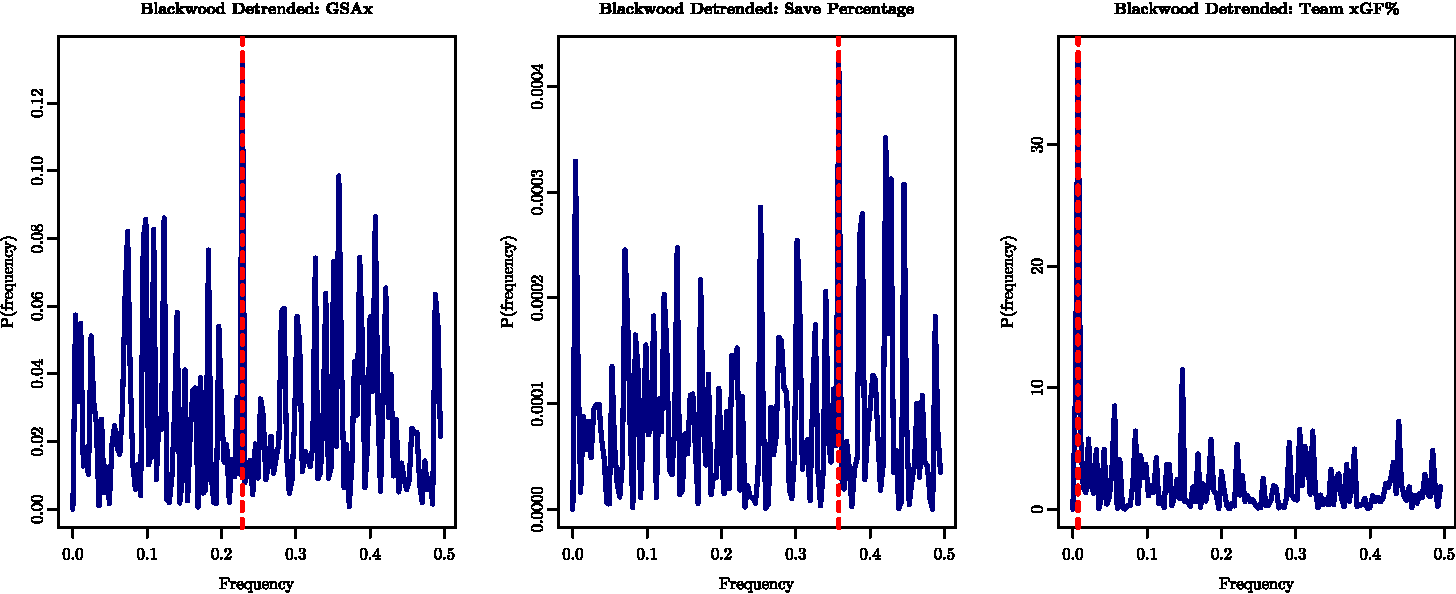
\includegraphics[width=\linewidth]{Homework7_files/figure-latex/p1-periodogram-blackwood-1} \end{center}

\begin{Shaded}
\begin{Highlighting}[]
\FunctionTok{with\_family}\NormalTok{(\{}
  \FunctionTok{plot\_periodograms}\NormalTok{(shesterkin\_detrended, }\StringTok{\textquotesingle{}Shesterkin Detrended\textquotesingle{}}\NormalTok{)}
\NormalTok{\})}
\end{Highlighting}
\end{Shaded}

\begin{center}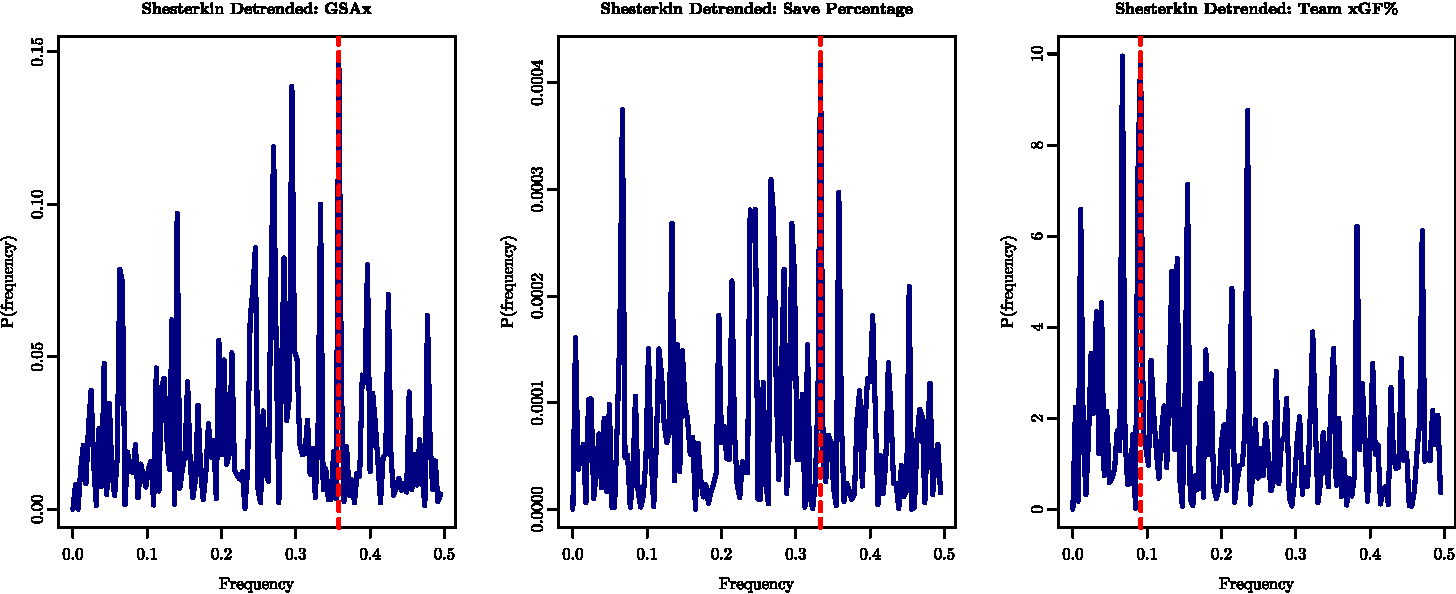
\includegraphics[width=\linewidth]{Homework7_files/figure-latex/p1-periodogram-shesterkin-1} \end{center}

For Blackwood, the largest periodogram peaks imply periods of about 4.38 games for \(\tilde{G}_t\), 2.79 games for \(\tilde{S}_t\), and 142.5 games for \(\tilde{X}_t\). For Shesterkin, they imply periods of about 2.79 games for \(\tilde{G}_t\), 3 games for \(\tilde{S}_t\), and 10.96 games for \(\tilde{X}_t\). These are not clear, stable, isolated seasonal periodicities. They are simply the largest sample periodogram peaks in noisy game-by-game data. Because \(t\) is a one-game-at-a-time career index, there is also no natural fixed calendar seasonality built into the time index. Therefore, I conclude that there is no meaningful seasonal pattern to model.

\newpage

\subsection{Problem 1 (e)}\label{problem-1-e}

\begin{problem}[Problem 1 (e)]
If there is seasonal pattern then model the overall behavior (trend and seasonality both) using the techniques learned in class.
\end{problem}

There is no meaningful seasonal pattern in part (d), and there is no nonconstant trend from part (c). Therefore, I do not fit a combined trend-and-seasonality model. Including harmonic terms or seasonal indicators would add parameters without a clear periodicity to justify them.

\newpage

\subsection{Problem 1 (f)}\label{problem-1-f}

\begin{problem}[Problem 1 (f)]
Use CCF between the response time series in your study and the predictors to see what if any lead-lag relation exists between the variables. State very clearly.
\end{problem}

The CCF step uses the detrended response \(\tilde{G}_t\) and the two detrended predictors \(\tilde{S}_t\) and \(\tilde{X}_t\). I use \texttt{ccf(predictor,\ response)}. In this convention, negative lags mean the predictor leads the response, so I rewrite those as positive predictor leads in games.

\begin{Shaded}
\begin{Highlighting}[]
\FunctionTok{with\_family}\NormalTok{(\{}
  \FunctionTok{plot\_goalie\_ccf}\NormalTok{(blackwood\_detrended, }\StringTok{\textquotesingle{}Blackwood\textquotesingle{}}\NormalTok{)}
\NormalTok{\})}
\end{Highlighting}
\end{Shaded}

\begin{center}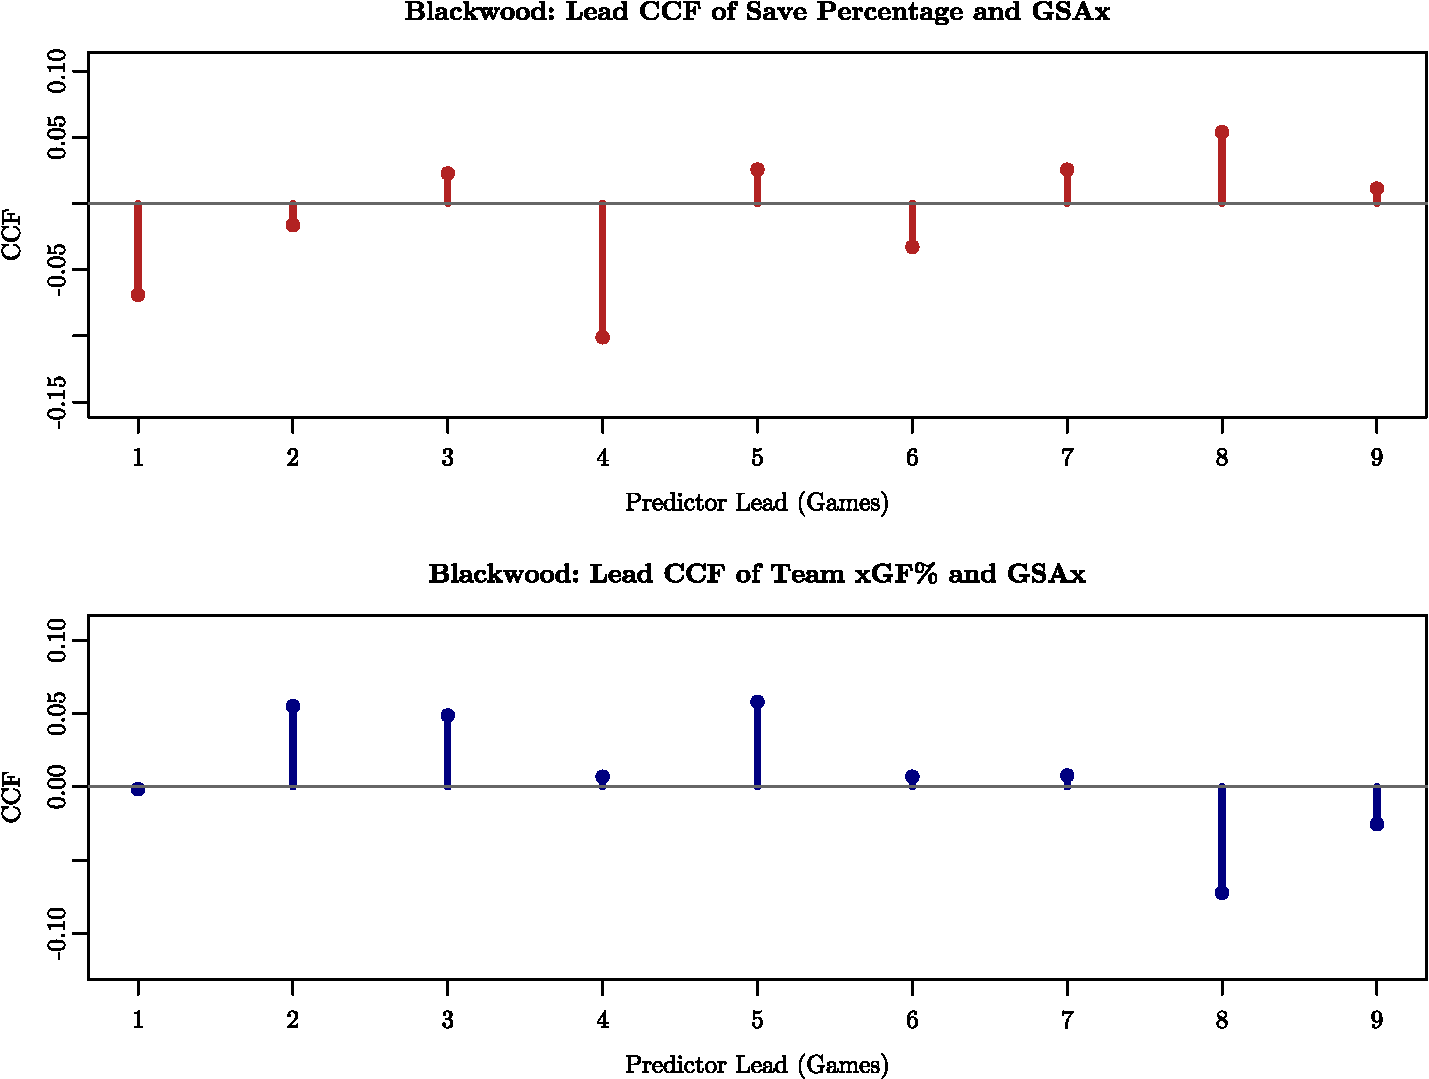
\includegraphics[width=\linewidth]{Homework7_files/figure-latex/p1-ccf-blackwood-1} \end{center}

For Blackwood, the largest save-percentage lead CCF magnitude over leads 1 through 9 is 0.1011 at lead 4, and the largest team-xGF\% lead CCF magnitude is 0.0723 at lead 8. The signs are negative for save percentage and negative for team xGF\%. These are weak lead-lag correlations, but they support carrying \(\tilde{S}_{t-4}\) and \(\tilde{X}_{t-8}\) into the time-series regression.

\begin{Shaded}
\begin{Highlighting}[]
\FunctionTok{with\_family}\NormalTok{(\{}
  \FunctionTok{plot\_goalie\_ccf}\NormalTok{(shesterkin\_detrended, }\StringTok{\textquotesingle{}Shesterkin\textquotesingle{}}\NormalTok{)}
\NormalTok{\})}
\end{Highlighting}
\end{Shaded}

\begin{center}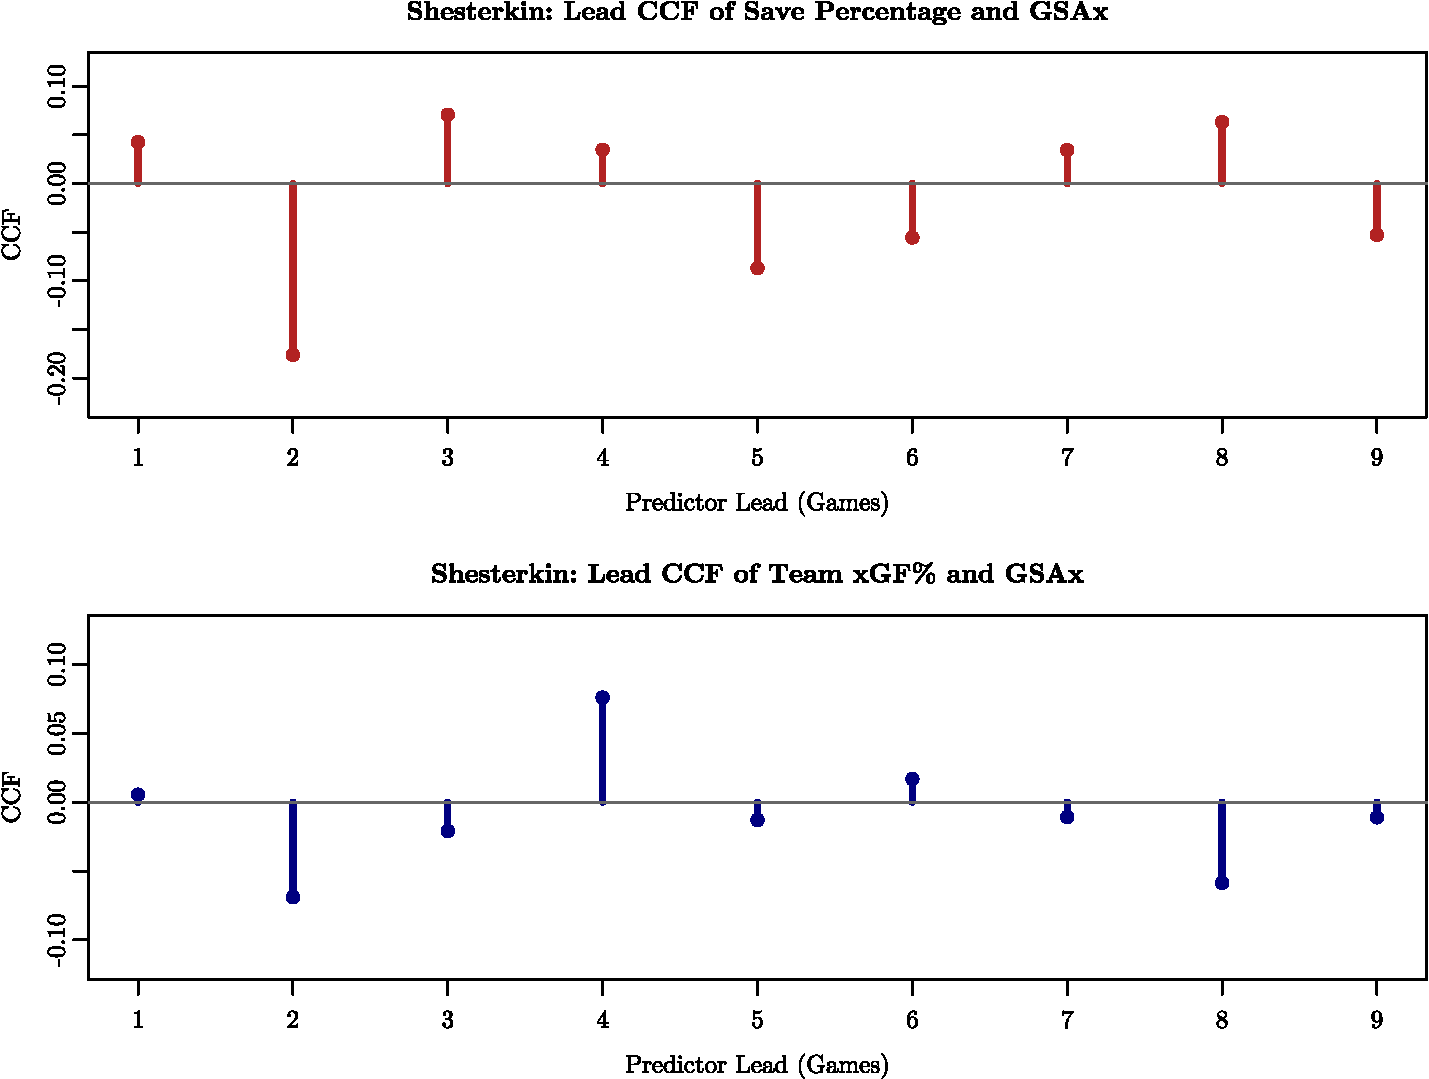
\includegraphics[width=\linewidth]{Homework7_files/figure-latex/p1-ccf-shesterkin-1} \end{center}

For Shesterkin, the largest save-percentage lead CCF magnitude is 0.1762 at lead 2, and the largest team-xGF\% lead CCF magnitude is 0.076 at lead 4. The save-percentage lead relation is more visible for Shesterkin than for Blackwood, while the team-xGF\% lead relation remains weak. I therefore carry \(\tilde{S}_{t-2}\) and \(\tilde{X}_{t-4}\) into the Shesterkin regression.

\newpage

\subsection{Problem 1 (g)}\label{problem-1-g}

\begin{problem}[Problem 1 (g)]
Use time series scatterplots to show over time relation between response and predictors. Clearly state the findings.
\end{problem}

\begin{Shaded}
\begin{Highlighting}[]
\FunctionTok{with\_family}\NormalTok{(\{}
  \FunctionTok{plot\_lagged\_scatter\_grid}\NormalTok{(blackwood\_detrended, }\StringTok{\textquotesingle{}Blackwood\textquotesingle{}}\NormalTok{, }\AttributeTok{predictor =} \StringTok{\textquotesingle{}sv\textquotesingle{}}\NormalTok{, }\AttributeTok{leads =} \DecValTok{1}\SpecialCharTok{:}\DecValTok{9}\NormalTok{)}
\NormalTok{\})}
\end{Highlighting}
\end{Shaded}

\begin{center}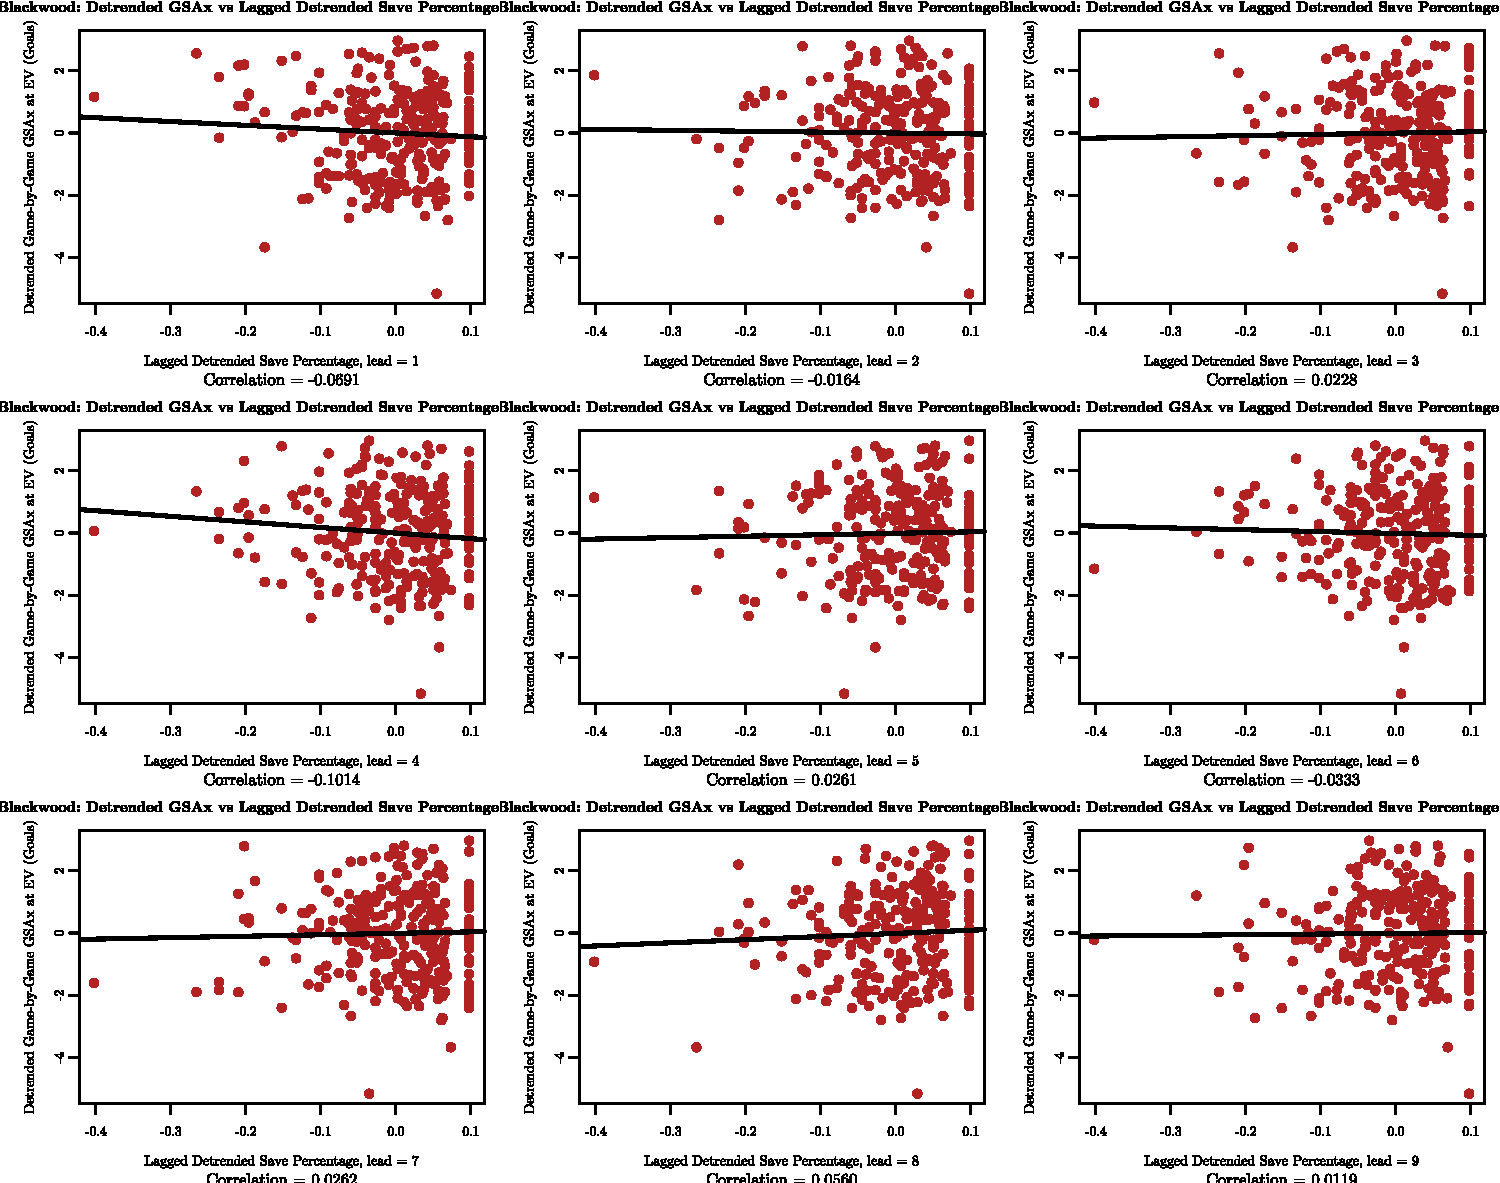
\includegraphics[width=\linewidth]{Homework7_files/figure-latex/p1-scatter-blackwood-sv-1} \end{center}

\begin{Shaded}
\begin{Highlighting}[]
\FunctionTok{with\_family}\NormalTok{(\{}
  \FunctionTok{plot\_lagged\_scatter\_grid}\NormalTok{(blackwood\_detrended, }\StringTok{\textquotesingle{}Blackwood\textquotesingle{}}\NormalTok{, }\AttributeTok{predictor =} \StringTok{\textquotesingle{}xgf\textquotesingle{}}\NormalTok{, }\AttributeTok{leads =} \DecValTok{1}\SpecialCharTok{:}\DecValTok{9}\NormalTok{)}
\NormalTok{\})}
\end{Highlighting}
\end{Shaded}

\begin{center}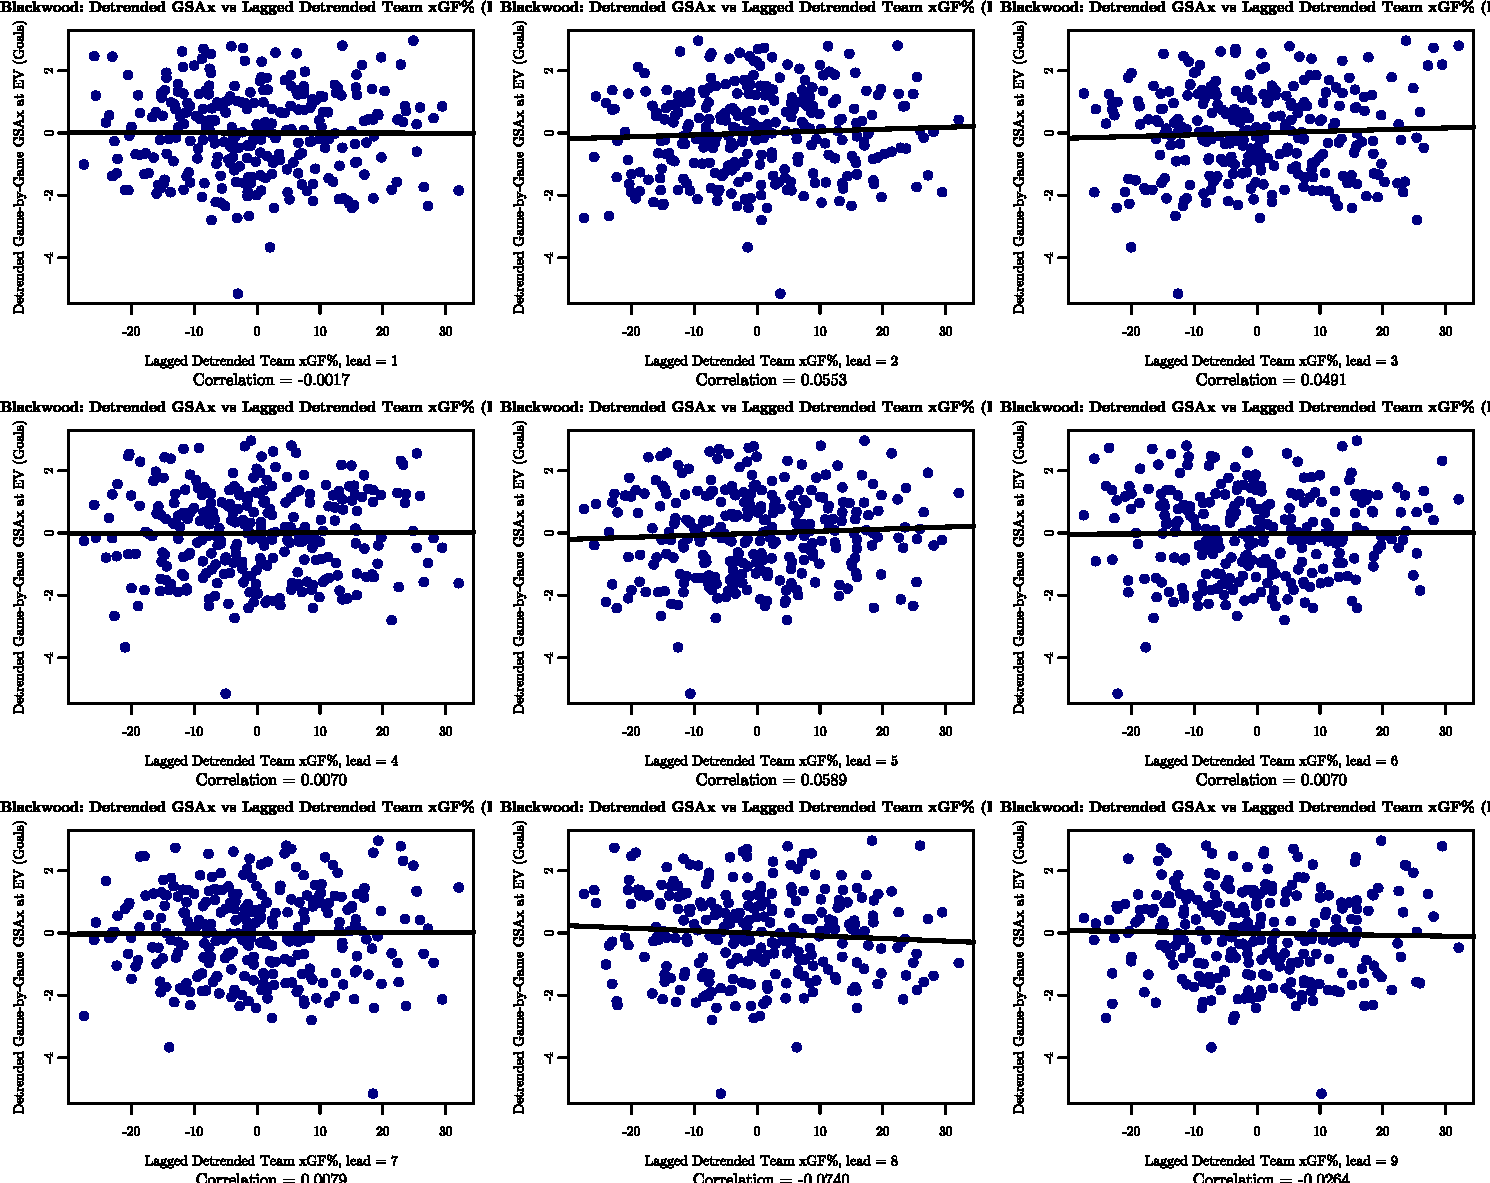
\includegraphics[width=\linewidth]{Homework7_files/figure-latex/p1-scatter-blackwood-xgf-1} \end{center}

The Blackwood detrended scatterplots are diffuse at almost every lead. The selected leads should therefore be interpreted as the strongest available lead-lag candidates, not as evidence of a strong deterministic relationship. This is important for the final interpretation: if the regression is weak, that is a real result rather than a failure to find a more complicated lead.

\begin{Shaded}
\begin{Highlighting}[]
\FunctionTok{with\_family}\NormalTok{(\{}
  \FunctionTok{plot\_lagged\_scatter\_grid}\NormalTok{(shesterkin\_detrended, }\StringTok{\textquotesingle{}Shesterkin\textquotesingle{}}\NormalTok{, }\AttributeTok{predictor =} \StringTok{\textquotesingle{}sv\textquotesingle{}}\NormalTok{, }\AttributeTok{leads =} \DecValTok{1}\SpecialCharTok{:}\DecValTok{9}\NormalTok{)}
\NormalTok{\})}
\end{Highlighting}
\end{Shaded}

\begin{center}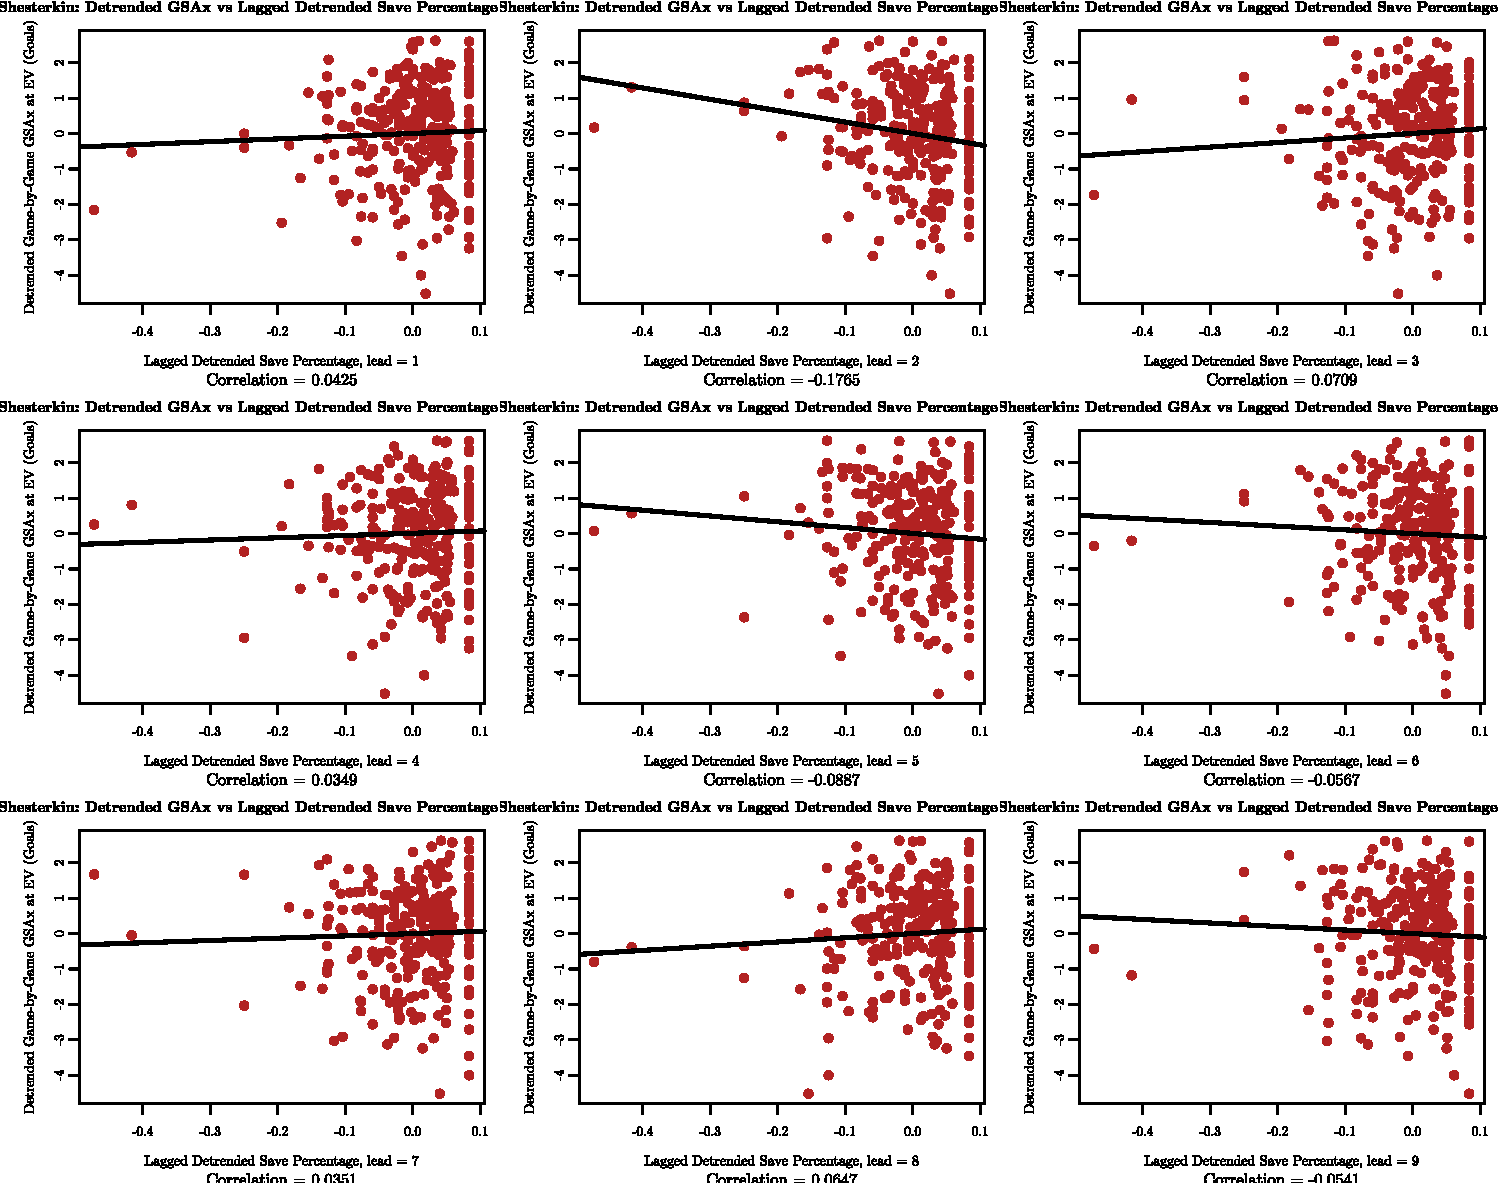
\includegraphics[width=\linewidth]{Homework7_files/figure-latex/p1-scatter-shesterkin-sv-1} \end{center}

\begin{Shaded}
\begin{Highlighting}[]
\FunctionTok{with\_family}\NormalTok{(\{}
  \FunctionTok{plot\_lagged\_scatter\_grid}\NormalTok{(shesterkin\_detrended, }\StringTok{\textquotesingle{}Shesterkin\textquotesingle{}}\NormalTok{, }\AttributeTok{predictor =} \StringTok{\textquotesingle{}xgf\textquotesingle{}}\NormalTok{, }\AttributeTok{leads =} \DecValTok{1}\SpecialCharTok{:}\DecValTok{9}\NormalTok{)}
\NormalTok{\})}
\end{Highlighting}
\end{Shaded}

\begin{center}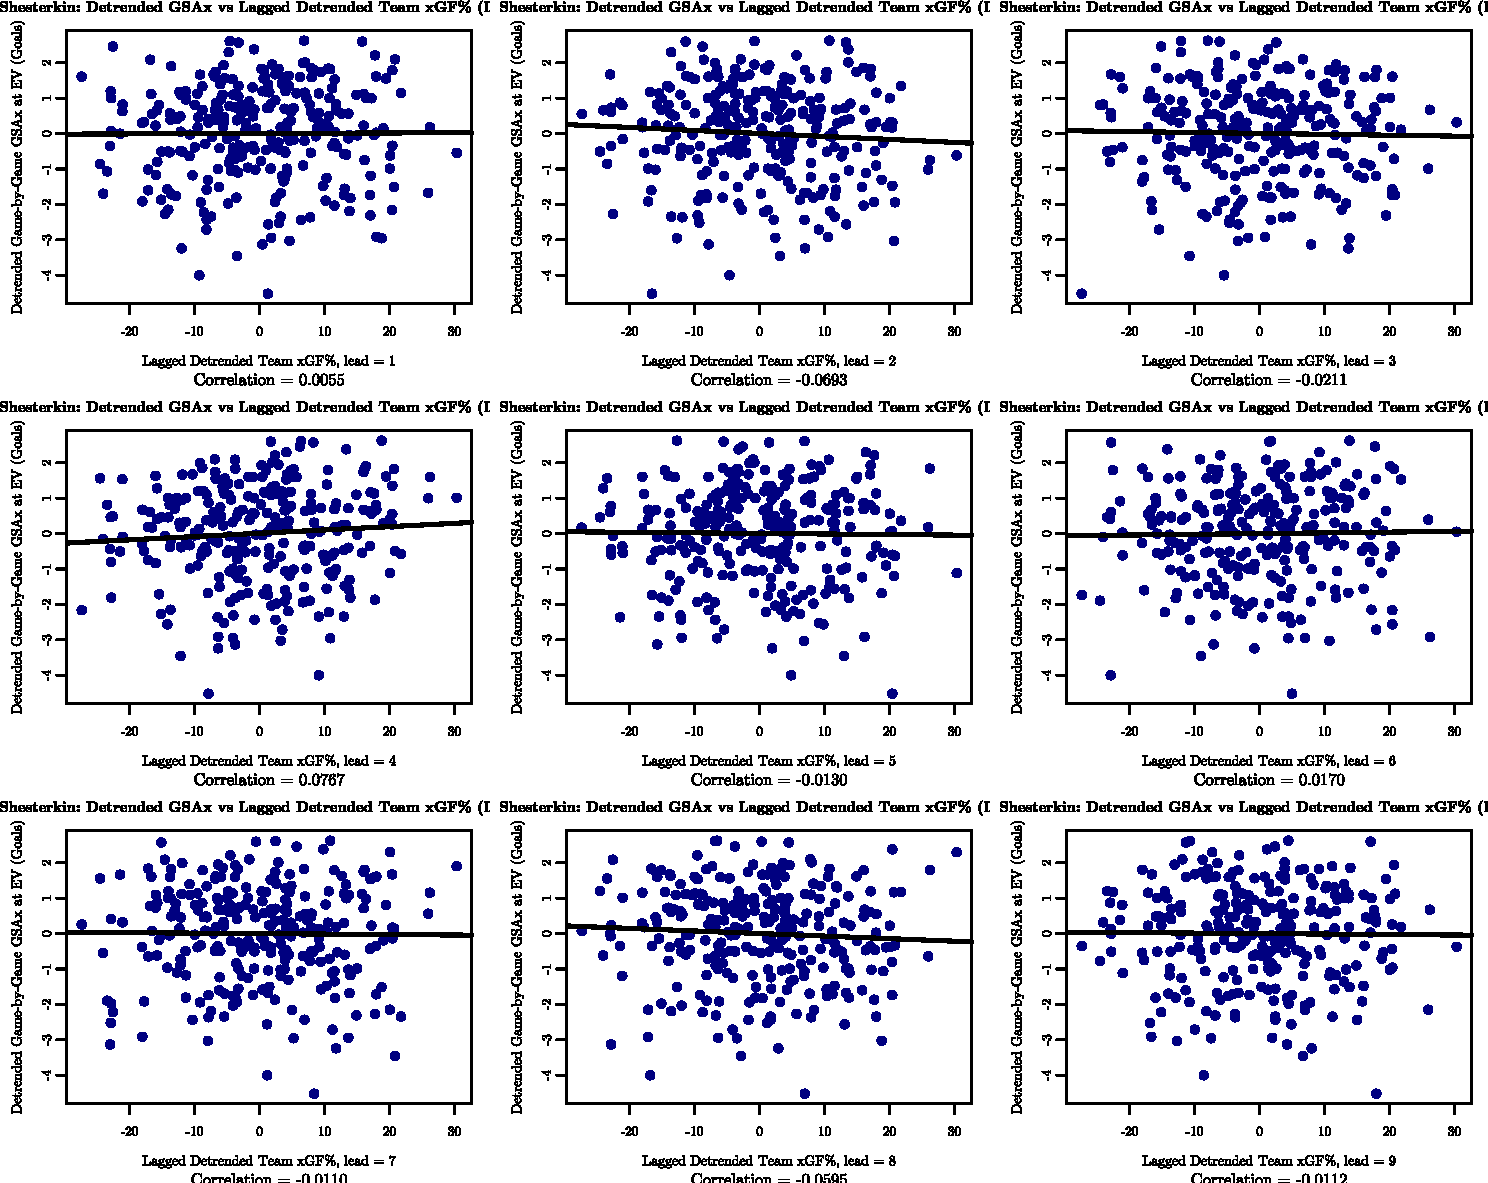
\includegraphics[width=\linewidth]{Homework7_files/figure-latex/p1-scatter-shesterkin-xgf-1} \end{center}

The Shesterkin detrended save-percentage scatterplots show the clearest relationship around the shorter leads, especially the two-game lead. The team-xGF\% plots remain much more scattered, so any team-context effect is weak in this direct lagged-regression setup.

\newpage

\subsection{Problem 1 (h)}\label{problem-1-h}

\begin{problem}[Problem 1 (h)]
If any transformations are needed for your data, please report that.
\end{problem}

I check the aligned detrended response and detrended predictors that enter the regression models. The goal is to decide whether the modeling variables need a variance-stabilizing transformation before fitting the final time-series regression.

\begin{Shaded}
\begin{Highlighting}[]
\FunctionTok{with\_family}\NormalTok{(\{}
\NormalTok{  op }\OtherTok{\textless{}{-}}\NormalTok{ graphics}\SpecialCharTok{::}\FunctionTok{par}\NormalTok{(}\AttributeTok{no.readonly =} \ConstantTok{TRUE}\NormalTok{)}
  \FunctionTok{on.exit}\NormalTok{(graphics}\SpecialCharTok{::}\FunctionTok{par}\NormalTok{(op), }\AttributeTok{add =} \ConstantTok{TRUE}\NormalTok{)}
\NormalTok{  graphics}\SpecialCharTok{::}\FunctionTok{par}\NormalTok{(}\AttributeTok{mfrow =} \FunctionTok{c}\NormalTok{(}\DecValTok{3}\NormalTok{, }\DecValTok{2}\NormalTok{), }\AttributeTok{mar =} \FunctionTok{c}\NormalTok{(}\FloatTok{4.0}\NormalTok{, }\FloatTok{4.4}\NormalTok{, }\FloatTok{2.6}\NormalTok{, }\FloatTok{1.0}\NormalTok{), }\AttributeTok{mgp =} \FunctionTok{c}\NormalTok{(}\FloatTok{2.2}\NormalTok{, }\FloatTok{0.7}\NormalTok{, }\DecValTok{0}\NormalTok{), }\AttributeTok{cex.main =} \FloatTok{0.92}\NormalTok{)}
\NormalTok{  astsa}\SpecialCharTok{::}\FunctionTok{tsplot}\NormalTok{(stats}\SpecialCharTok{::}\FunctionTok{ts}\NormalTok{(blackwood\_raw\_reg}\SpecialCharTok{$}\NormalTok{data}\SpecialCharTok{$}\NormalTok{g, }\AttributeTok{start =} \FunctionTok{min}\NormalTok{(blackwood\_raw\_reg}\SpecialCharTok{$}\NormalTok{data}\SpecialCharTok{$}\NormalTok{t), }\AttributeTok{frequency =} \DecValTok{1}\NormalTok{), }\AttributeTok{main =} \StringTok{\textquotesingle{}Blackwood: Aligned Detrended GSAx Response\textquotesingle{}}\NormalTok{, }\AttributeTok{xlab =} \StringTok{\textquotesingle{}Career Game Number (t)\textquotesingle{}}\NormalTok{, }\AttributeTok{ylab =} \StringTok{\textquotesingle{}Detrended GSAx (Goals)\textquotesingle{}}\NormalTok{, }\AttributeTok{col =} \StringTok{\textquotesingle{}darkgreen\textquotesingle{}}\NormalTok{, }\AttributeTok{lwd =} \DecValTok{2}\NormalTok{)}
\NormalTok{  astsa}\SpecialCharTok{::}\FunctionTok{tsplot}\NormalTok{(stats}\SpecialCharTok{::}\FunctionTok{ts}\NormalTok{(shesterkin\_raw\_reg}\SpecialCharTok{$}\NormalTok{data}\SpecialCharTok{$}\NormalTok{g, }\AttributeTok{start =} \FunctionTok{min}\NormalTok{(shesterkin\_raw\_reg}\SpecialCharTok{$}\NormalTok{data}\SpecialCharTok{$}\NormalTok{t), }\AttributeTok{frequency =} \DecValTok{1}\NormalTok{), }\AttributeTok{main =} \StringTok{\textquotesingle{}Shesterkin: Aligned Detrended GSAx Response\textquotesingle{}}\NormalTok{, }\AttributeTok{xlab =} \StringTok{\textquotesingle{}Career Game Number (t)\textquotesingle{}}\NormalTok{, }\AttributeTok{ylab =} \StringTok{\textquotesingle{}Detrended GSAx (Goals)\textquotesingle{}}\NormalTok{, }\AttributeTok{col =} \StringTok{\textquotesingle{}darkgreen\textquotesingle{}}\NormalTok{, }\AttributeTok{lwd =} \DecValTok{2}\NormalTok{)}
\NormalTok{  astsa}\SpecialCharTok{::}\FunctionTok{tsplot}\NormalTok{(stats}\SpecialCharTok{::}\FunctionTok{ts}\NormalTok{(blackwood\_raw\_reg}\SpecialCharTok{$}\NormalTok{data}\SpecialCharTok{$}\NormalTok{sv, }\AttributeTok{start =} \FunctionTok{min}\NormalTok{(blackwood\_raw\_reg}\SpecialCharTok{$}\NormalTok{data}\SpecialCharTok{$}\NormalTok{t), }\AttributeTok{frequency =} \DecValTok{1}\NormalTok{), }\AttributeTok{main =} \StringTok{\textquotesingle{}Blackwood: Lagged Detrended Save Percentage\textquotesingle{}}\NormalTok{, }\AttributeTok{xlab =} \StringTok{\textquotesingle{}Career Game Number (t)\textquotesingle{}}\NormalTok{, }\AttributeTok{ylab =} \StringTok{\textquotesingle{}S\textasciitilde{}(t{-}4)\textquotesingle{}}\NormalTok{, }\AttributeTok{col =} \StringTok{\textquotesingle{}firebrick\textquotesingle{}}\NormalTok{, }\AttributeTok{lwd =} \DecValTok{2}\NormalTok{)}
\NormalTok{  astsa}\SpecialCharTok{::}\FunctionTok{tsplot}\NormalTok{(stats}\SpecialCharTok{::}\FunctionTok{ts}\NormalTok{(shesterkin\_raw\_reg}\SpecialCharTok{$}\NormalTok{data}\SpecialCharTok{$}\NormalTok{sv, }\AttributeTok{start =} \FunctionTok{min}\NormalTok{(shesterkin\_raw\_reg}\SpecialCharTok{$}\NormalTok{data}\SpecialCharTok{$}\NormalTok{t), }\AttributeTok{frequency =} \DecValTok{1}\NormalTok{), }\AttributeTok{main =} \StringTok{\textquotesingle{}Shesterkin: Lagged Detrended Save Percentage\textquotesingle{}}\NormalTok{, }\AttributeTok{xlab =} \StringTok{\textquotesingle{}Career Game Number (t)\textquotesingle{}}\NormalTok{, }\AttributeTok{ylab =} \StringTok{\textquotesingle{}S\textasciitilde{}(t{-}2)\textquotesingle{}}\NormalTok{, }\AttributeTok{col =} \StringTok{\textquotesingle{}firebrick\textquotesingle{}}\NormalTok{, }\AttributeTok{lwd =} \DecValTok{2}\NormalTok{)}
\NormalTok{  astsa}\SpecialCharTok{::}\FunctionTok{tsplot}\NormalTok{(stats}\SpecialCharTok{::}\FunctionTok{ts}\NormalTok{(blackwood\_raw\_reg}\SpecialCharTok{$}\NormalTok{data}\SpecialCharTok{$}\NormalTok{xgf, }\AttributeTok{start =} \FunctionTok{min}\NormalTok{(blackwood\_raw\_reg}\SpecialCharTok{$}\NormalTok{data}\SpecialCharTok{$}\NormalTok{t), }\AttributeTok{frequency =} \DecValTok{1}\NormalTok{), }\AttributeTok{main =} \StringTok{\textquotesingle{}Blackwood: Lagged Detrended Team xGF\%\textquotesingle{}}\NormalTok{, }\AttributeTok{xlab =} \StringTok{\textquotesingle{}Career Game Number (t)\textquotesingle{}}\NormalTok{, }\AttributeTok{ylab =} \StringTok{\textquotesingle{}X\textasciitilde{}(t{-}8)\textquotesingle{}}\NormalTok{, }\AttributeTok{col =} \StringTok{\textquotesingle{}navy\textquotesingle{}}\NormalTok{, }\AttributeTok{lwd =} \DecValTok{2}\NormalTok{)}
\NormalTok{  astsa}\SpecialCharTok{::}\FunctionTok{tsplot}\NormalTok{(stats}\SpecialCharTok{::}\FunctionTok{ts}\NormalTok{(shesterkin\_raw\_reg}\SpecialCharTok{$}\NormalTok{data}\SpecialCharTok{$}\NormalTok{xgf, }\AttributeTok{start =} \FunctionTok{min}\NormalTok{(shesterkin\_raw\_reg}\SpecialCharTok{$}\NormalTok{data}\SpecialCharTok{$}\NormalTok{t), }\AttributeTok{frequency =} \DecValTok{1}\NormalTok{), }\AttributeTok{main =} \StringTok{\textquotesingle{}Shesterkin: Lagged Detrended Team xGF\%\textquotesingle{}}\NormalTok{, }\AttributeTok{xlab =} \StringTok{\textquotesingle{}Career Game Number (t)\textquotesingle{}}\NormalTok{, }\AttributeTok{ylab =} \StringTok{\textquotesingle{}X\textasciitilde{}(t{-}4)\textquotesingle{}}\NormalTok{, }\AttributeTok{col =} \StringTok{\textquotesingle{}navy\textquotesingle{}}\NormalTok{, }\AttributeTok{lwd =} \DecValTok{2}\NormalTok{)}
\NormalTok{\})}
\end{Highlighting}
\end{Shaded}

\begin{center}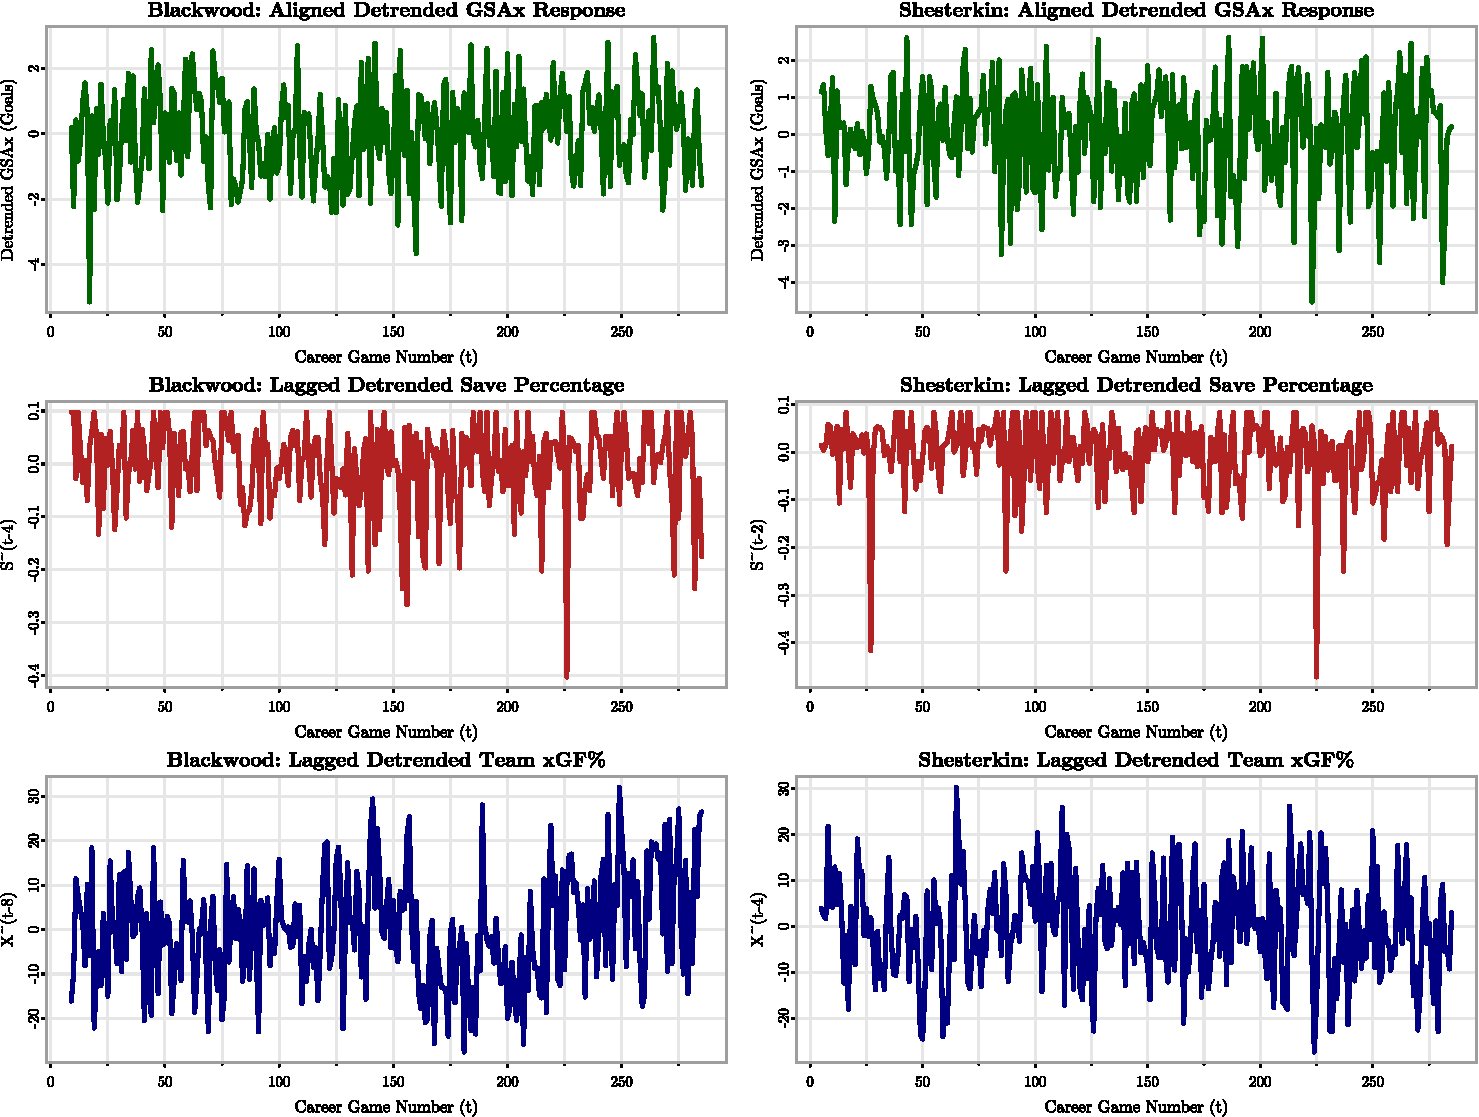
\includegraphics[width=\linewidth]{Homework7_files/figure-latex/p1-transformation-plots-1} \end{center}

\begin{center}
\scriptsize
\begin{table}[H]

\caption{\label{tab:p1-blackwood-diag-table}Blackwood aligned variable diagnostics}
\centering
\begin{tabular}[t]{ccccccc}
\toprule
Series & Mean & Min & Max & 1st-Half Var. & 2nd-Half Var. & 2nd/1st\\
\midrule
$\tilde{G}_t$ & -0.0101 & -5.1500 & 2.9613 & 1.9890 & 1.8449 & 0.9276\\
$\tilde{S}_{t-4}$ & -0.0002 & -0.4023 & 0.0977 & 0.0049 & 0.0075 & 1.5534\\
$\tilde{X}_{t-8}$ & -0.1352 & -27.5615 & 32.0656 & 118.8624 & 193.0579 & 1.6242\\
\bottomrule
\end{tabular}
\end{table}
\normalsize
\end{center}

\begin{center}
\scriptsize
\begin{table}[H]

\caption{\label{tab:p1-blackwood-transform-table}Blackwood shifted log and Box-Cox comparison}
\centering
\begin{tabular}[t]{cccccc}
\toprule
Series & Shift & $\hat{\lambda}$ & Raw & Shifted Log & Shifted Box-Cox\\
\midrule
$\tilde{G}_t$ & 6.1500 & 1.6711 & 0.9276 & 0.7313 & 0.9781\\
$\tilde{S}_{t-4}$ & 1.4023 & 1.9999 & 1.5534 & 1.6996 & 1.4385\\
$\tilde{X}_{t-8}$ & 28.5615 & 0.8931 & 1.6242 & 1.9295 & 1.6173\\
\bottomrule
\end{tabular}
\end{table}
\normalsize
\end{center}

For Blackwood, the detrended response variance ratio is 0.9276. The shifted Box-Cox response transformation improves this to 0.9781, while the shifted log makes it worse at 0.7313. For the predictors, the ratios are 1.5534 for \(\tilde{S}_{t-4}\) and 1.6242 for \(\tilde{X}_{t-8}\). The Box-Cox transformation does move \(\tilde{S}_{t-4}\) from 1.5534 to 1.4385, so it improves the raw ratio in the numerical sense. However, the transformed ratio is still not especially close to 1, while the transformed response ratio is very close to 1. Transforming \(\tilde{S}_{t-4}\) would also make the predictor harder to interpret because it would no longer mean a save-percentage deviation from the goalie's average. Since the improvement for \(\tilde{S}_{t-4}\) is incomplete and has an interpretability cost, I keep the predictors in detrended but untransformed units. Therefore, I transform only Blackwood's detrended response:
\[
Y^{(B)}_t
= \frac{\left(\tilde{G}_t + 6.15\right)^{1.6711} - 1}{1.6711}.
\]
This transformed response is on the shifted Box-Cox detrended-GSAx scale, while \(\tilde{S}_{t-4}\) remains in proportion-deviation units and \(\tilde{X}_{t-8}\) remains in percentage-point-deviation units.

\begin{center}
\scriptsize
\begin{table}[H]

\caption{\label{tab:p1-shesterkin-diag-table}Shesterkin aligned variable diagnostics}
\centering
\begin{tabular}[t]{ccccccc}
\toprule
Series & Mean & Min & Max & 1st-Half Var. & 2nd-Half Var. & 2nd/1st\\
\midrule
$\tilde{G}_t$ & 0.0085 & -4.5209 & 2.6241 & 1.4834 & 2.1938 & 1.4789\\
$\tilde{S}_{t-2}$ & -0.0001 & -0.4718 & 0.0837 & 0.0048 & 0.0062 & 1.2784\\
$\tilde{X}_{t-4}$ & -0.0569 & -27.3865 & 30.3506 & 116.5492 & 131.4910 & 1.1282\\
\bottomrule
\end{tabular}
\end{table}
\normalsize
\end{center}

\begin{center}
\scriptsize
\begin{table}[H]

\caption{\label{tab:p1-shesterkin-transform-table}Shesterkin shifted log and Box-Cox comparison}
\centering
\begin{tabular}[t]{cccccc}
\toprule
Series & Shift & $\hat{\lambda}$ & Raw & Shifted Log & Shifted Box-Cox\\
\midrule
$\tilde{G}_t$ & 5.5209 & 1.9999 & 1.4789 & 1.9401 & 1.3248\\
$\tilde{S}_{t-2}$ & 1.4718 & 1.9999 & 1.2784 & 1.3061 & 1.2579\\
$\tilde{X}_{t-4}$ & 28.3865 & 0.6331 & 1.1282 & 1.3331 & 1.1530\\
\bottomrule
\end{tabular}
\end{table}
\normalsize
\end{center}

For Shesterkin, the detrended response variance ratio is 1.4789. The shifted Box-Cox response transformation improves this to 1.3248, while the shifted log makes it worse at 1.9401. For the predictors, the raw ratios are already milder: 1.2784 for \(\tilde{S}_{t-2}\) and 1.1282 for \(\tilde{X}_{t-4}\). Therefore, I transform only Shesterkin's detrended response:
\[
Y^{(S)}_t
= \frac{\left(\tilde{G}_t + 5.5209\right)^{1.9999} - 1}{1.9999}.
\]
This transformed response is on the shifted Box-Cox detrended-GSAx scale, while \(\tilde{S}_{t-2}\) remains in proportion-deviation units and \(\tilde{X}_{t-4}\) remains in percentage-point-deviation units.

\newpage

\subsection{Problem 1 (i)}\label{problem-1-i}

\begin{problem}[Problem 1 (i)]
Fit a time series regression model for your response variable using the predictors.
\end{problem}

The final time-series regression models use only the detrended lagged predictors from the CCF step:
\[
\text{Response}_t = \beta_0 + \beta_1 \tilde{S}_{t-h_S} + \beta_2 \tilde{X}_{t-h_X} + W_t.
\]
For both goalies, the response is the shifted Box-Cox transformed version of \(\tilde{G}_t\) from part (h), while the predictors stay detrended but untransformed. For Blackwood, the model is
\[
Y^{(B)}_t = \beta_0 + \beta_1 \tilde{S}_{t-4} + \beta_2 \tilde{X}_{t-8} + W_t.
\]
The fitted model is
\[
\widehat{Y}^{(B)}_t = 12.172950 - 5.523364 \tilde{S}_{t-4} - 0.032082 \tilde{X}_{t-8}.
\]
Here, \(Y^{(B)}_t\) is Blackwood's shifted Box-Cox transformed detrended game-by-game even-strength GSAx at career game \(t\), \(\tilde{S}_{t-4}\) is Blackwood's even-strength save percentage four games earlier after subtracting Blackwood's average save percentage, and \(\tilde{X}_{t-8}\) is Blackwood's team even-strength xGF\% eight games earlier after subtracting Blackwood's average team xGF\%. Because the largest lag is 8, the aligned regression sample uses \(t = 9,\ldots,285\), so it contains \(n=277\) observations.

To write this on the original GSAx scale, I reverse the shifted Box-Cox transformation and add back the fitted average level from part (c). Since
\[
Y^{(B)}_t
= \frac{\left(\tilde{G}_t + 6.15\right)^{1.6711} - 1}{1.6711},
\]
the fitted model on the original GSAx scale is
\[
\widehat{G}_t
=
\left[
1.6711
\left(12.172950 - 5.523364 \tilde{S}_{t-4} - 0.032082 \tilde{X}_{t-8}\right)
+ 1
\right]^{1/1.6711}
- 6.15
- 0.0400.
\]
This reversed equation is the interpretable fitted-value equation for \(G_t\), measured in goals. The final - 0.0400 term applies Blackwood's fitted average GSAx level from part (c).

\begin{Shaded}
\begin{Highlighting}[]
\NormalTok{blackwood\_reg}\SpecialCharTok{$}\NormalTok{fit}
\end{Highlighting}
\end{Shaded}

\begin{verbatim}
## 
## Call:
## stats::lm(formula = g ~ sv + xgf, data = blackwood_trans_data)
## 
## Coefficients:
## (Intercept)           sv          xgf  
##    12.17295     -5.52336     -0.03208
\end{verbatim}

\begin{Shaded}
\begin{Highlighting}[]
\FunctionTok{summary}\NormalTok{(blackwood\_reg}\SpecialCharTok{$}\NormalTok{fit)}
\end{Highlighting}
\end{Shaded}

\begin{verbatim}
## 
## Call:
## stats::lm(formula = g ~ sv + xgf, data = blackwood_trans_data)
## 
## Residuals:
##      Min       1Q   Median       3Q      Max 
## -12.1746  -3.6083  -0.0597   3.1739  11.6372 
## 
## Coefficients:
##             Estimate Std. Error t value            Pr(>|t|)    
## (Intercept) 12.17295    0.27638  44.045 <0.0000000000000002 ***
## sv          -5.52336    3.51831  -1.570               0.118    
## xgf         -0.03208    0.02223  -1.443               0.150    
## ---
## Signif. codes:  0 '***' 0.001 '**' 0.01 '*' 0.05 '.' 0.1 ' ' 1
## 
## Residual standard error: 4.6 on 274 degrees of freedom
## Multiple R-squared:  0.01547,    Adjusted R-squared:  0.008282 
## F-statistic: 2.153 on 2 and 274 DF,  p-value: 0.1182
\end{verbatim}

\begin{center}
\scriptsize
\begin{table}[H]

\caption{\label{tab:p1-blackwood-reg-comparison}Blackwood detrended-response and transformed-detrended-response regression comparison}
\centering
\resizebox{\linewidth}{!}{\begin{tabular}[t]{ccccccc}
\toprule
Model & \# Parameters & $R_a^2$ & $p_F$ & AIC & AICc & BIC\\
\midrule
Detrended response & 3 & 0.0078 & 0.1267 & 3.5017 & 1.6643 & 3.5540\\
Shifted Box-Cox detrended response & 3 & 0.0083 & 0.1182 & 5.9078 & 4.0704 & 5.9601\\
\bottomrule
\end{tabular}}
\end{table}
\normalsize
\end{center}

\begin{center}
\scriptsize
\begin{table}[H]

\caption{\label{tab:p1-blackwood-reg-coef}Blackwood time-series regression coefficients}
\centering
\begin{tabular}[t]{ccccc}
\toprule
Term & Estimate & Std. Error & t Value & P-value\\
\midrule
Intercept & 12.172950 & 0.276376 & 44.044906 & <0.0001\\
$\tilde{S}_{t-4}$ & -5.523364 & 3.518306 & -1.569893 & 0.1176\\
$\tilde{X}_{t-8}$ & -0.032082 & 0.022230 & -1.443157 & 0.1501\\
\bottomrule
\end{tabular}
\end{table}
\normalsize
\end{center}

\begin{center}
\scriptsize
\begin{table}[H]

\caption{\label{tab:p1-blackwood-reg-fit}Blackwood time-series regression fit criteria}
\centering
\begin{tabular}[t]{cccccc}
\toprule
\# Parameters & $R_a^2$ & $p_F$ & AIC & AICc & BIC\\
\midrule
3 & 0.0083 & 0.1182 & 5.9078 & 4.0704 & 5.9601\\
\bottomrule
\end{tabular}
\end{table}
\normalsize
\end{center}

For Blackwood, a 0.01 increase in \(\tilde{S}_{t-4}\), meaning save percentage 0.01 above its fitted average level four games earlier, is associated with a change of -0.0552 shifted Box-Cox units in current \(Y^{(B)}_t\), holding \(\tilde{X}_{t-8}\) fixed. A one-percentage-point increase in \(\tilde{X}_{t-8}\), meaning team xGF\% one percentage point above its fitted average level eight games earlier, is associated with a change of -0.0321 shifted Box-Cox units in current \(Y^{(B)}_t\), holding \(\tilde{S}_{t-4}\) fixed. The coefficient table gives the separate \(t\)-tests for the intercept, \(\tilde{S}_{t-4}\), and \(\tilde{X}_{t-8}\); for the two predictors, these p-values test whether that lagged detrended predictor contributes to current transformed detrended GSAx after the other lagged detrended predictor is already in the model. The adjusted \(R^2\) is 0.0083, so after accounting for the number of predictors, the model explains essentially none of the game-to-game variation in Blackwood's transformed detrended GSAx. The residual standard error is 4.5995 transformed-response units, meaning a typical fitted residual is about 4.5995 units on the shifted Box-Cox scale. The overall F-test p-value is 0.1182; this tests \(H_0:\beta_1=\beta_2=0\), so it asks whether the lagged detrended save percentage and lagged detrended team xGF\% variables jointly improve the model over an intercept-only model. Since this p-value is larger than 0.05, I do not have strong evidence that the two lagged detrended predictors jointly explain Blackwood's current transformed detrended GSAx. This is a weak model, but that weakness is informative: the selected lagged predictors do not explain much of Blackwood's next-game transformed detrended GSAx variation.

For Shesterkin, the model is
\[
Y^{(S)}_t = \beta_0 + \beta_1 \tilde{S}_{t-2} + \beta_2 \tilde{X}_{t-4} + W_t.
\]
The fitted model is
\[
\widehat{Y}^{(S)}_t = 15.700904 - 17.000714 \tilde{S}_{t-2} + 0.054228 \tilde{X}_{t-4}.
\]
Here, \(Y^{(S)}_t\) is Shesterkin's shifted Box-Cox transformed detrended game-by-game even-strength GSAx at career game \(t\), \(\tilde{S}_{t-2}\) is Shesterkin's even-strength save percentage two games earlier after subtracting Shesterkin's average save percentage, and \(\tilde{X}_{t-4}\) is the Rangers' even-strength xGF\% four games earlier after subtracting Shesterkin's average team xGF\%. Because the largest lag is 4, the aligned regression sample uses \(t = 5,\ldots,285\), so it contains \(n=281\) observations. To write this on the original GSAx scale, I reverse the shifted Box-Cox transformation and add back the fitted average level from part (c). Since
\[
Y^{(S)}_t
= \frac{\left(\tilde{G}_t + 5.5209\right)^{1.9999} - 1}{1.9999},
\]
the fitted model on the original GSAx scale is
\[
\widehat{G}_t
=
\left[
1.9999
\left(15.700904 - 17.000714 \tilde{S}_{t-2} + 0.054228 \tilde{X}_{t-4}\right)
+ 1
\right]^{1/1.9999}
- 5.5209
+ 0.2329.
\]
This reversed equation is the interpretable fitted-value equation for \(G_t\), measured in goals. The final + 0.2329 term applies Shesterkin's fitted average GSAx level from part (c). The effects of \(\tilde{S}_{t-2}\) and \(\tilde{X}_{t-4}\) are no longer additive constants in goals after reversing the transformation; they act through the nonlinear inverse Box-Cox expression.

\begin{center}
\scriptsize
\begin{table}[H]

\caption{\label{tab:p1-shesterkin-reg-comparison}Shesterkin detrended-response and transformed-detrended-response regression comparison}
\centering
\resizebox{\linewidth}{!}{\begin{tabular}[t]{ccccccc}
\toprule
Model & \# Parameters & $R_a^2$ & $p_F$ & AIC & AICc & BIC\\
\midrule
Detrended response & 3 & 0.0296 & 0.0057 & 3.4325 & 1.5951 & 3.4843\\
Shifted Box-Cox detrended response & 3 & 0.0324 & 0.0038 & 6.7467 & 4.9094 & 6.7985\\
\bottomrule
\end{tabular}}
\end{table}
\normalsize
\end{center}

\begin{Shaded}
\begin{Highlighting}[]
\NormalTok{shesterkin\_reg}\SpecialCharTok{$}\NormalTok{fit}
\end{Highlighting}
\end{Shaded}

\begin{verbatim}
## 
## Call:
## stats::lm(formula = g ~ sv + xgf, data = shesterkin_trans_data)
## 
## Coefficients:
## (Intercept)           sv          xgf  
##    15.70090    -17.00071      0.05423
\end{verbatim}

\begin{Shaded}
\begin{Highlighting}[]
\FunctionTok{summary}\NormalTok{(shesterkin\_reg}\SpecialCharTok{$}\NormalTok{fit)}
\end{Highlighting}
\end{Shaded}

\begin{verbatim}
## 
## Call:
## stats::lm(formula = g ~ sv + xgf, data = shesterkin_trans_data)
## 
## Residuals:
##      Min       1Q   Median       3Q      Max 
## -15.6589  -5.7656   0.0314   4.3300  17.2547 
## 
## Coefficients:
##              Estimate Std. Error t value            Pr(>|t|)    
## (Intercept)  15.70090    0.41745  37.612 <0.0000000000000002 ***
## sv          -17.00071    5.61708  -3.027              0.0027 ** 
## xgf           0.05423    0.03756   1.444              0.1500    
## ---
## Signif. codes:  0 '***' 0.001 '**' 0.01 '*' 0.05 '.' 0.1 ' ' 1
## 
## Residual standard error: 6.998 on 278 degrees of freedom
## Multiple R-squared:  0.03928,    Adjusted R-squared:  0.03237 
## F-statistic: 5.683 on 2 and 278 DF,  p-value: 0.003811
\end{verbatim}

\begin{center}
\scriptsize
\begin{table}[H]

\caption{\label{tab:p1-shesterkin-reg-coef}Shesterkin time-series regression coefficients}
\centering
\begin{tabular}[t]{ccccc}
\toprule
Term & Estimate & Std. Error & t Value & P-value\\
\midrule
Intercept & 15.700904 & 0.417445 & 37.611879 & <0.0001\\
$\tilde{S}_{t-2}$ & -17.000714 & 5.617085 & -3.026608 & 0.0027\\
$\tilde{X}_{t-4}$ & 0.054228 & 0.037562 & 1.443679 & 0.1500\\
\bottomrule
\end{tabular}
\end{table}
\normalsize
\end{center}

\begin{center}
\scriptsize
\begin{table}[H]

\caption{\label{tab:p1-shesterkin-reg-fit}Shesterkin time-series regression fit criteria}
\centering
\begin{tabular}[t]{cccccc}
\toprule
\# Parameters & $R_a^2$ & $p_F$ & AIC & AICc & BIC\\
\midrule
3 & 0.0324 & 0.0038 & 6.7467 & 4.9094 & 6.7985\\
\bottomrule
\end{tabular}
\end{table}
\normalsize
\end{center}

For Shesterkin, a 0.01 increase in \(\tilde{S}_{t-2}\), meaning save percentage 0.01 above its fitted average level two games earlier, is associated with a change of -0.17 shifted Box-Cox units in current \(Y^{(S)}_t\), holding \(\tilde{X}_{t-4}\) fixed. A one-percentage-point increase in \(\tilde{X}_{t-4}\), meaning team xGF\% one percentage point above its fitted average level four games earlier, is associated with a change of 0.0542 shifted Box-Cox units in current \(Y^{(S)}_t\), holding \(\tilde{S}_{t-2}\) fixed. The coefficient table gives the separate \(t\)-tests for the intercept, \(\tilde{S}_{t-2}\), and \(\tilde{X}_{t-4}\); for the two predictors, these p-values test whether that lagged detrended predictor contributes to current transformed detrended GSAx after the other lagged detrended predictor is already in the model. The adjusted \(R^2\) is 0.0324, so after accounting for the number of predictors, the model explains only a small amount of the game-to-game variation in Shesterkin's transformed detrended GSAx. The residual standard error is 6.9976 transformed-response units, meaning a typical fitted residual is about 6.9976 units on the shifted Box-Cox scale. The overall F-test p-value is 0.0038; this tests \(H_0:\beta_1=\beta_2=0\), so it asks whether the lagged detrended save percentage and lagged detrended team xGF\% variables jointly improve the model over an intercept-only model. Since this p-value is below 0.05, I reject that joint null hypothesis and conclude that the two lagged detrended predictors jointly improve the model statistically. However, the adjusted \(R^2\) is still small, so the statistically significant result does not mean that the model explains a large share of Shesterkin's game-to-game transformed detrended GSAx variation.

\newpage

\section{Problem 2}\label{problem-2}

\begin{problem}[Problem 2]
Answer the following questions about your data project.
\end{problem}

\newpage

\subsection{Problem 2 (a)}\label{problem-2-a}

\begin{problem}[Problem 2 (a)]
Plot the residuals from your TS regression and comment on any interesting features.
\end{problem}

The residuals come from the time-series regression models in Problem 1:
\[
Y^{(B)}_t = \beta_0 + \beta_1 \tilde{S}_{t-4} + \beta_2 \tilde{X}_{t-8} + W_t
\]
for Blackwood and
\[
Y^{(S)}_t = \beta_0 + \beta_1 \tilde{S}_{t-2} + \beta_2 \tilde{X}_{t-4} + W_t
\]
for Shesterkin. Both residual series are measured on shifted Box-Cox detrended-GSAx response scales.

\begin{Shaded}
\begin{Highlighting}[]
\FunctionTok{with\_family}\NormalTok{(\{}
\NormalTok{  op }\OtherTok{\textless{}{-}}\NormalTok{ graphics}\SpecialCharTok{::}\FunctionTok{par}\NormalTok{(}\AttributeTok{no.readonly =} \ConstantTok{TRUE}\NormalTok{)}
  \FunctionTok{on.exit}\NormalTok{(graphics}\SpecialCharTok{::}\FunctionTok{par}\NormalTok{(op), }\AttributeTok{add =} \ConstantTok{TRUE}\NormalTok{)}
\NormalTok{  graphics}\SpecialCharTok{::}\FunctionTok{par}\NormalTok{(}\AttributeTok{mfrow =} \FunctionTok{c}\NormalTok{(}\DecValTok{2}\NormalTok{, }\DecValTok{1}\NormalTok{), }\AttributeTok{mar =} \FunctionTok{c}\NormalTok{(}\FloatTok{4.2}\NormalTok{, }\FloatTok{4.8}\NormalTok{, }\FloatTok{3.0}\NormalTok{, }\FloatTok{1.2}\NormalTok{), }\AttributeTok{mgp =} \FunctionTok{c}\NormalTok{(}\FloatTok{2.2}\NormalTok{, }\FloatTok{0.7}\NormalTok{, }\DecValTok{0}\NormalTok{), }\AttributeTok{cex.main =} \FloatTok{1.05}\NormalTok{)}
\NormalTok{  astsa}\SpecialCharTok{::}\FunctionTok{tsplot}\NormalTok{(stats}\SpecialCharTok{::}\FunctionTok{ts}\NormalTok{(blackwood\_resid, }\AttributeTok{start =} \FunctionTok{min}\NormalTok{(blackwood\_reg}\SpecialCharTok{$}\NormalTok{data}\SpecialCharTok{$}\NormalTok{t), }\AttributeTok{frequency =} \DecValTok{1}\NormalTok{), }\AttributeTok{main =} \StringTok{\textquotesingle{}Blackwood: Residuals from TS Regression\textquotesingle{}}\NormalTok{, }\AttributeTok{xlab =} \StringTok{\textquotesingle{}Career Game Number (t)\textquotesingle{}}\NormalTok{, }\AttributeTok{ylab =} \StringTok{\textquotesingle{}Residuals (Transformed Scale)\textquotesingle{}}\NormalTok{, }\AttributeTok{col =} \StringTok{\textquotesingle{}black\textquotesingle{}}\NormalTok{, }\AttributeTok{lwd =} \DecValTok{2}\NormalTok{)}
\NormalTok{  graphics}\SpecialCharTok{::}\FunctionTok{abline}\NormalTok{(}\AttributeTok{h =} \DecValTok{0}\NormalTok{, }\AttributeTok{lty =} \DecValTok{2}\NormalTok{, }\AttributeTok{col =} \StringTok{\textquotesingle{}gray40\textquotesingle{}}\NormalTok{)}
\NormalTok{  astsa}\SpecialCharTok{::}\FunctionTok{tsplot}\NormalTok{(stats}\SpecialCharTok{::}\FunctionTok{ts}\NormalTok{(shesterkin\_resid, }\AttributeTok{start =} \FunctionTok{min}\NormalTok{(shesterkin\_reg}\SpecialCharTok{$}\NormalTok{data}\SpecialCharTok{$}\NormalTok{t), }\AttributeTok{frequency =} \DecValTok{1}\NormalTok{), }\AttributeTok{main =} \StringTok{\textquotesingle{}Shesterkin: Residuals from TS Regression\textquotesingle{}}\NormalTok{, }\AttributeTok{xlab =} \StringTok{\textquotesingle{}Career Game Number (t)\textquotesingle{}}\NormalTok{, }\AttributeTok{ylab =} \StringTok{\textquotesingle{}Residuals (Transformed Scale)\textquotesingle{}}\NormalTok{, }\AttributeTok{col =} \StringTok{\textquotesingle{}black\textquotesingle{}}\NormalTok{, }\AttributeTok{lwd =} \DecValTok{2}\NormalTok{)}
\NormalTok{  graphics}\SpecialCharTok{::}\FunctionTok{abline}\NormalTok{(}\AttributeTok{h =} \DecValTok{0}\NormalTok{, }\AttributeTok{lty =} \DecValTok{2}\NormalTok{, }\AttributeTok{col =} \StringTok{\textquotesingle{}gray40\textquotesingle{}}\NormalTok{)}
\NormalTok{\})}
\end{Highlighting}
\end{Shaded}

\begin{center}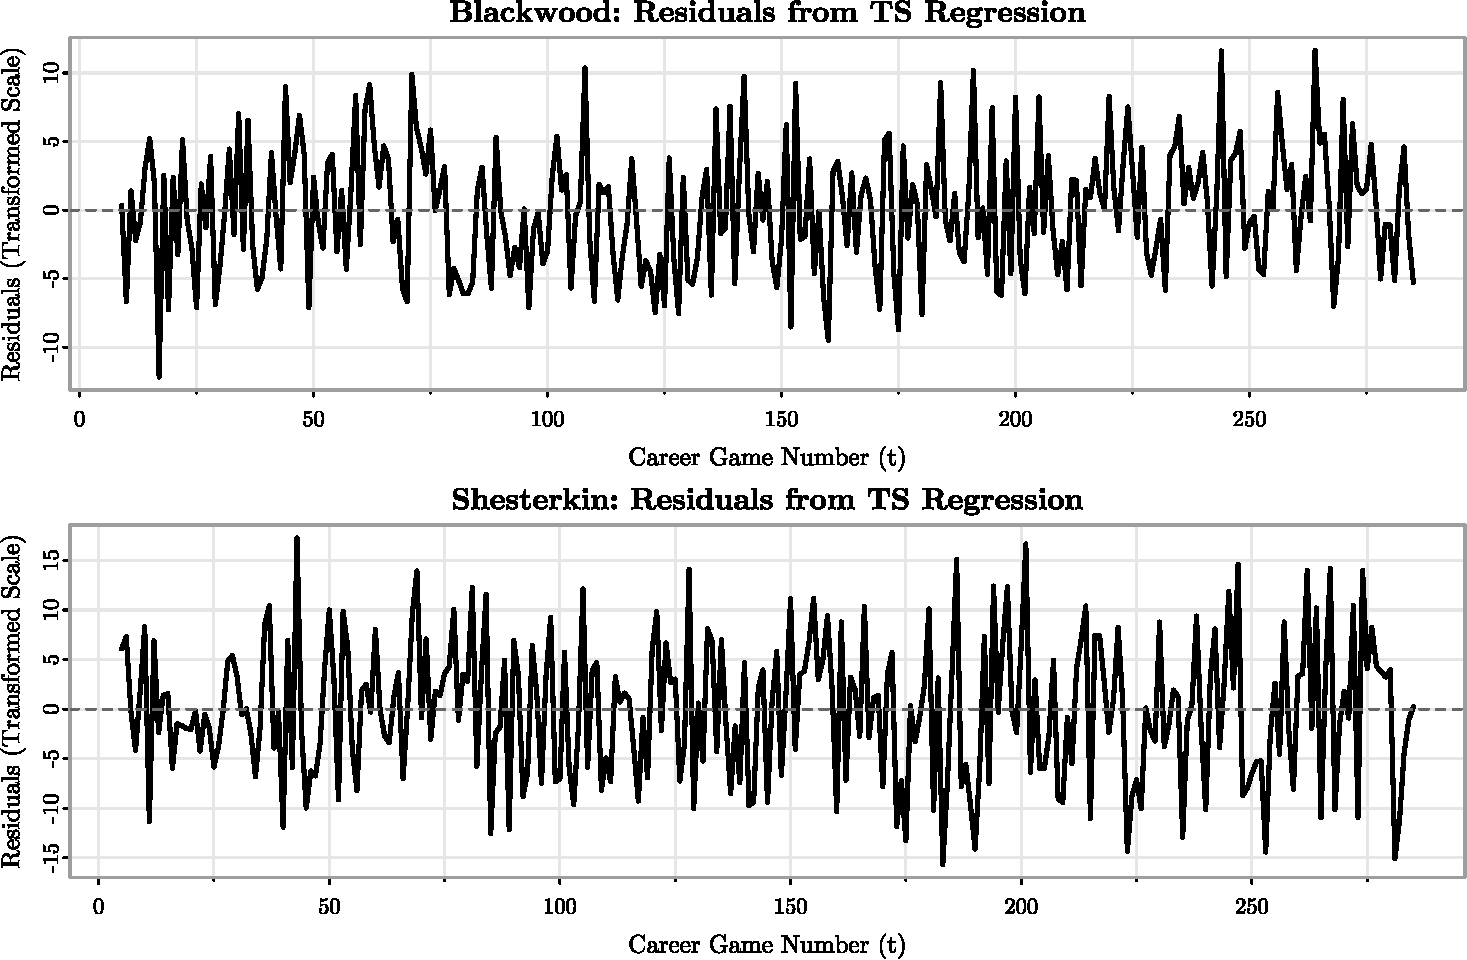
\includegraphics[width=\linewidth]{Homework7_files/figure-latex/p2-residual-plots-1} \end{center}

For Blackwood, the residual series is measured on the shifted Box-Cox detrended-response scale and has sample mean 0. The plot fluctuates around zero and does not show a sustained linear or nonlinear trend. There is no visible seasonal pattern because the residual spikes do not repeat with a fixed game periodicity. The residual range is -12.1746 to 11.6372 transformed-response units, for a total range of 23.8118. The spread looks fairly stable over time, so there is no strong visual evidence of heteroscedasticity. There are isolated positive and negative spikes, but there is no clear volatility clustering. For Shesterkin, the residual series is also measured on the shifted Box-Cox detrended-response scale and has sample mean 0. The plot also fluctuates around zero with no visible deterministic trend. There is no clear seasonal pattern. The residual range is -15.6589 to 17.2547 transformed-response units, for a total range of 32.9135. The spread is reasonably stable, and further ACF/PACF and ARMA/ARIMA checks will be useful in determining if this is already white noise.

\newpage

\subsection{Problem 2 (b)}\label{problem-2-b}

\begin{problem}[Problem 2 (b)]
Plot ACF and PACF of these residuals to discuss the dependence pattern.
\end{problem}

\begin{Shaded}
\begin{Highlighting}[]
\FunctionTok{with\_family}\NormalTok{(\{}
\NormalTok{  op }\OtherTok{\textless{}{-}}\NormalTok{ graphics}\SpecialCharTok{::}\FunctionTok{par}\NormalTok{(}\AttributeTok{no.readonly =} \ConstantTok{TRUE}\NormalTok{)}
  \FunctionTok{on.exit}\NormalTok{(graphics}\SpecialCharTok{::}\FunctionTok{par}\NormalTok{(op), }\AttributeTok{add =} \ConstantTok{TRUE}\NormalTok{)}
\NormalTok{  graphics}\SpecialCharTok{::}\FunctionTok{par}\NormalTok{(}\AttributeTok{mfrow =} \FunctionTok{c}\NormalTok{(}\DecValTok{2}\NormalTok{, }\DecValTok{2}\NormalTok{), }\AttributeTok{mar =} \FunctionTok{c}\NormalTok{(}\FloatTok{4.0}\NormalTok{, }\FloatTok{4.2}\NormalTok{, }\FloatTok{3.0}\NormalTok{, }\FloatTok{1.0}\NormalTok{), }\AttributeTok{mgp =} \FunctionTok{c}\NormalTok{(}\FloatTok{2.2}\NormalTok{, }\FloatTok{0.7}\NormalTok{, }\DecValTok{0}\NormalTok{), }\AttributeTok{cex.main =} \FloatTok{1.0}\NormalTok{)}
\NormalTok{  stats}\SpecialCharTok{::}\FunctionTok{acf}\NormalTok{(blackwood\_resid, }\AttributeTok{lag.max =} \DecValTok{24}\NormalTok{, }\AttributeTok{main =} \StringTok{\textquotesingle{}Blackwood Residual ACF\textquotesingle{}}\NormalTok{, }\AttributeTok{col =} \StringTok{\textquotesingle{}navy\textquotesingle{}}\NormalTok{, }\AttributeTok{lwd =} \DecValTok{2}\NormalTok{)}
\NormalTok{  stats}\SpecialCharTok{::}\FunctionTok{pacf}\NormalTok{(blackwood\_resid, }\AttributeTok{lag.max =} \DecValTok{24}\NormalTok{, }\AttributeTok{main =} \StringTok{\textquotesingle{}Blackwood Residual PACF\textquotesingle{}}\NormalTok{, }\AttributeTok{col =} \StringTok{\textquotesingle{}firebrick\textquotesingle{}}\NormalTok{, }\AttributeTok{lwd =} \DecValTok{2}\NormalTok{)}
\NormalTok{  stats}\SpecialCharTok{::}\FunctionTok{acf}\NormalTok{(shesterkin\_resid, }\AttributeTok{lag.max =} \DecValTok{24}\NormalTok{, }\AttributeTok{main =} \StringTok{\textquotesingle{}Shesterkin Residual ACF\textquotesingle{}}\NormalTok{, }\AttributeTok{col =} \StringTok{\textquotesingle{}navy\textquotesingle{}}\NormalTok{, }\AttributeTok{lwd =} \DecValTok{2}\NormalTok{)}
\NormalTok{  stats}\SpecialCharTok{::}\FunctionTok{pacf}\NormalTok{(shesterkin\_resid, }\AttributeTok{lag.max =} \DecValTok{24}\NormalTok{, }\AttributeTok{main =} \StringTok{\textquotesingle{}Shesterkin Residual PACF\textquotesingle{}}\NormalTok{, }\AttributeTok{col =} \StringTok{\textquotesingle{}firebrick\textquotesingle{}}\NormalTok{, }\AttributeTok{lwd =} \DecValTok{2}\NormalTok{)}
\NormalTok{\})}
\end{Highlighting}
\end{Shaded}

\begin{center}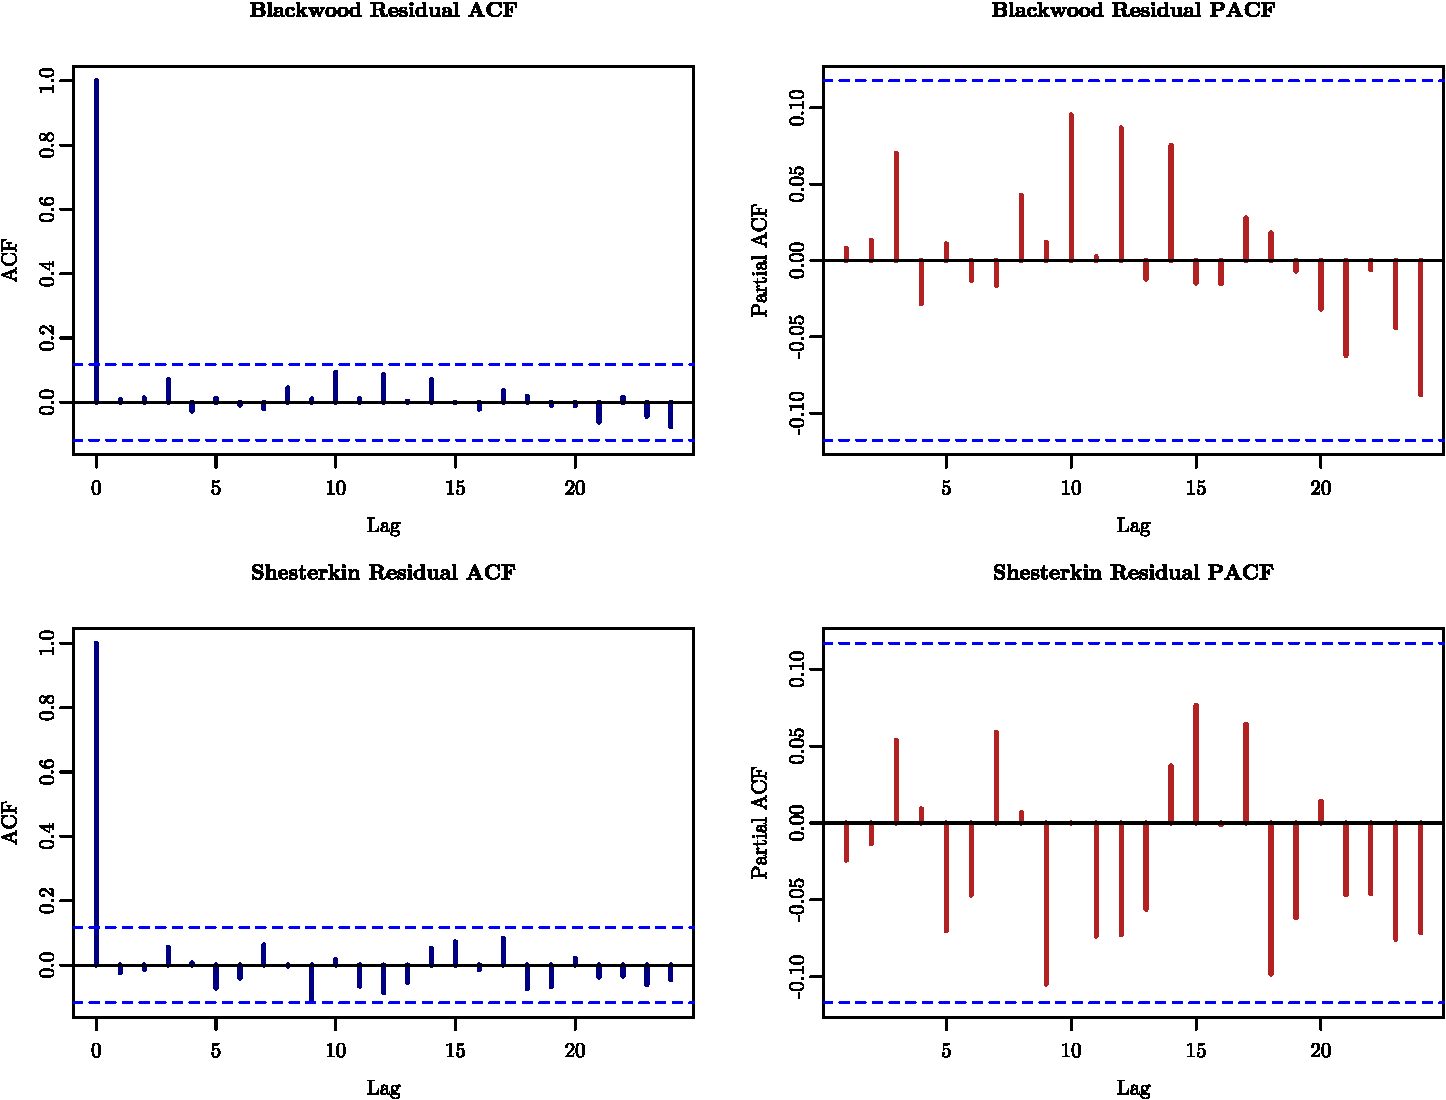
\includegraphics[width=\linewidth]{Homework7_files/figure-latex/p2-acf-pacf-1} \end{center}

For white noise, the ACF should have value 1 at lag 0 and should be close to 0 at all nonzero lags, with most sample spikes staying inside the approximate significance bounds. The PACF of white noise should behave similarly: there should be no systematic pattern and no long sequence of important partial autocorrelations. For both Blackwood and Shesterkin, the residual ACF and PACF are fairly close to that white-noise pattern. They do not show a long slow decay, and most nonzero-lag spikes are small. This means a white-noise residual model is plausible, although I still compare low-order ARMA models in part (c). Overall, if we must, this suggests trying low-order ARMA models.

\newpage

\subsection{Problem 2 (c)}\label{problem-2-c}

\begin{problem}[Problem 2 (c)]
Using steps for ARMA(p,q) fit show the model fit. Justify your choice using ACF and PACF of residuals from TS regression. Report the fitted model, \(\hat{\sigma}^2_W\), number of predictors and AIC for each model.
\end{problem}

I fit the same set of low-order ARMA models to the Blackwood and Shesterkin regression residuals. Let \(R_t\) denote the residual series from the transformed-detrended-response regression. The ARMA model form is
\[
R_t = \phi_1 R_{t-1} + \cdots + \phi_p R_{t-p}
      + W_t + \theta_1 W_{t-1} + \cdots + \theta_q W_{t-q}.
\]
The residuals are already centered near 0 by construction, so the question here is whether any AR or MA lag terms remain useful after fitting the time-series regression. The number of predictors in the table is \(p+q\), the number of AR and MA lag terms.

\begin{center}
\scriptsize
\begin{table}[H]

\caption{\label{tab:p2-arma-blackwood-table}Blackwood ARMA candidate models for TS-regression residuals}
\centering
\begin{tabular}[t]{ccccccc}
\toprule
Model & p & d & q & \# Predictors & $\hat{\sigma}_W^2$ & AIC\\
\midrule
ARIMA(0,0,0) & 0 & 0 & 0 & 0 & 20.9264 & 1630.452\\
ARIMA(1,0,0) & 1 & 0 & 0 & 1 & 20.9250 & 1632.434\\
ARIMA(0,0,1) & 0 & 0 & 1 & 1 & 20.9251 & 1632.435\\
ARIMA(1,0,1) & 1 & 0 & 1 & 2 & 20.9251 & 1634.435\\
ARIMA(2,0,0) & 2 & 0 & 0 & 2 & 20.9213 & 1634.385\\
\addlinespace
ARIMA(0,0,2) & 0 & 0 & 2 & 2 & 20.9216 & 1634.390\\
ARIMA(2,0,1) & 2 & 0 & 1 & 3 & 20.8340 & 1635.258\\
ARIMA(1,0,2) & 1 & 0 & 2 & 3 & 20.8514 & 1635.479\\
\bottomrule
\end{tabular}
\end{table}
\normalsize
\end{center}

The lowest-AIC Blackwood ARMA candidate is ARIMA(0,0,0), with \(\hat{\sigma}_W^2 = 20.9264\) and AIC \(= 1630.4519\). Its coefficient table is:

\begin{center}
\scriptsize
\begin{table}[H]

\caption{\label{tab:p2-arma-blackwood-coef}Blackwood ARIMA(0,0,0) coefficient estimates}
\centering
\begin{tabular}[t]{cc}
\toprule
Term & Estimate\\
\midrule
No AR or MA coefficients & NA\\
\bottomrule
\end{tabular}
\end{table}
\normalsize
\end{center}

Thus, with \(R_t^{(B)}\) denoting Blackwood's residual series from the transformed-detrended-response regression, the fitted Blackwood ARMA residual model is
\[
R_t^{(B)} = W_t.
\]

For Blackwood, the residual plots and ACF/PACF already suggested weak dependence, and I select ARIMA(0,0,0) by AIC. Since the selected model has no AR terms and no MA terms, it is a white-noise residual model rather than an additional dependence model. In other words, after accounting for lagged detrended save percentage and lagged detrended team xGF\% in the transformed-detrended-response regression, this ARMA step does not find useful remaining game-to-game dependence in Blackwood's residuals.

\begin{center}
\scriptsize
\begin{table}[H]

\caption{\label{tab:p2-arma-shesterkin-table}Shesterkin ARMA candidate models for TS-regression residuals}
\centering
\begin{tabular}[t]{ccccccc}
\toprule
Model & p & d & q & \# Predictors & $\hat{\sigma}_W^2$ & AIC\\
\midrule
ARIMA(0,0,0) & 0 & 0 & 0 & 0 & 48.4430 & 1889.833\\
ARIMA(1,0,0) & 1 & 0 & 0 & 1 & 48.4148 & 1891.670\\
ARIMA(0,0,1) & 0 & 0 & 1 & 1 & 48.4141 & 1891.666\\
ARIMA(1,0,1) & 1 & 0 & 1 & 2 & 48.4134 & 1893.661\\
ARIMA(2,0,0) & 2 & 0 & 0 & 2 & 48.4057 & 1893.617\\
\addlinespace
ARIMA(0,0,2) & 0 & 0 & 2 & 2 & 48.4088 & 1893.635\\
ARIMA(2,0,1) & 2 & 0 & 1 & 3 & 48.3750 & 1895.440\\
ARIMA(1,0,2) & 1 & 0 & 2 & 3 & 48.3812 & 1895.476\\
\bottomrule
\end{tabular}
\end{table}
\normalsize
\end{center}

The lowest-AIC Shesterkin ARMA candidate is ARIMA(0,0,0), with \(\hat{\sigma}_W^2 = 48.443\) and AIC \(= 1889.8327\). Its coefficient table is:

\begin{center}
\scriptsize
\begin{table}[H]

\caption{\label{tab:p2-arma-shesterkin-coef}Shesterkin ARIMA(0,0,0) coefficient estimates}
\centering
\begin{tabular}[t]{cc}
\toprule
Term & Estimate\\
\midrule
No AR or MA coefficients & NA\\
\bottomrule
\end{tabular}
\end{table}
\normalsize
\end{center}

Thus, with \(R_t^{(S)}\) denoting Shesterkin's residual series from the transformed-detrended-response regression, the fitted Shesterkin ARMA residual model is
\[
R_t^{(S)} = W_t.
\]

For Shesterkin, I also select ARIMA(0,0,0) by AIC. Since the selected model has no AR terms and no MA terms, it is also a white-noise residual model. This agrees with the part (b) ACF/PACF discussion: Shesterkin's residuals are close enough to white noise that the low-order ARMA candidates do not improve the residual model by AIC. This model is on the shifted Box-Cox detrended-response residual scale.

\newpage

\subsection{Problem 2 (d)}\label{problem-2-d}

\begin{problem}[Problem 2 (d)]
Repeat the ARMA-model comparison for ARIMA(p,d,q).
\end{problem}

The residual plots and ADF results from Problem 1 suggest that differencing is not required. However, to answer the ARIMA part directly, I fit first-differenced ARIMA candidates with \(d=1\), using the same \(p,q\) combinations as in the ARMA comparison:
\[
\nabla R_t = (1-B)R_t \sim ARMA(p,q).
\]
I then compare these first-differenced models to the selected ARMA(0,0) residual model from part (c), because ARMA(0,0) was the best non-differenced residual model for both goalies.

\begin{center}
\scriptsize
\begin{table}[H]

\caption{\label{tab:p2-arima-blackwood-table}Blackwood ARIMA candidate models for TS-regression residuals}
\centering
\begin{tabular}[t]{ccccccc}
\toprule
Model & p & d & q & \# Predictors & $\hat{\sigma}_W^2$ & AIC\\
\midrule
ARIMA(0,1,0) & 0 & 1 & 0 & 0 & 41.5682 & 1813.998\\
ARIMA(1,1,0) & 1 & 1 & 0 & 1 & 31.0311 & 1735.603\\
ARIMA(0,1,1) & 0 & 1 & 1 & 1 & 21.1021 & 1632.004\\
ARIMA(1,1,1) & 1 & 1 & 1 & 2 & 21.1021 & 1633.991\\
ARIMA(2,1,0) & 2 & 1 & 0 & 2 & 26.7430 & 1696.855\\
\addlinespace
ARIMA(0,1,2) & 0 & 1 & 2 & 2 & 21.1021 & 1633.991\\
ARIMA(2,1,1) & 2 & 1 & 1 & 3 & 21.1023 & 1635.990\\
ARIMA(1,1,2) & 1 & 1 & 2 & 3 & 21.0921 & 1635.892\\
\bottomrule
\end{tabular}
\end{table}
\normalsize
\end{center}

For Blackwood, the best first-differenced ARIMA candidate is ARIMA(0,1,1), with \(\hat{\sigma}_W^2 = 21.1021\) and AIC \(= 1632.004\). The ARMA(0,0) model from part (c) had \(\hat{\sigma}_W^2 = 20.9264\) and AIC \(= 1630.4519\). Therefore, for Blackwood, the first-differenced ARIMA choice has a higher AIC than ARMA(0,0), with an AIC difference of 1.5521. Its coefficient estimates are:

\begin{center}
\scriptsize
\begin{table}[H]

\caption{\label{tab:p2-arima-blackwood-coef}Blackwood ARIMA(0,1,1) coefficient estimates}
\centering
\begin{tabular}[t]{cc}
\toprule
Term & Estimate\\
\midrule
ma1 & -0.977753\\
\bottomrule
\end{tabular}
\end{table}
\normalsize
\end{center}

Thus, with \(R_t^{(B)}\) denoting Blackwood's residual series from the transformed-detrended-response regression, the fitted Blackwood ARIMA residual model is
\[
\nabla R_t^{(B)} = W_t - 0.977753 W_{t-1}.
\]

\begin{center}
\scriptsize
\begin{table}[H]

\caption{\label{tab:p2-arima-shesterkin-table}Shesterkin ARIMA candidate models for TS-regression residuals}
\centering
\begin{tabular}[t]{ccccccc}
\toprule
Model & p & d & q & \# Predictors & $\hat{\sigma}_W^2$ & AIC\\
\midrule
ARIMA(0,1,0) & 0 & 1 & 0 & 0 & 99.4429 & 2084.489\\
ARIMA(1,1,0) & 1 & 1 & 0 & 1 & 73.9446 & 2003.828\\
ARIMA(0,1,1) & 0 & 1 & 1 & 1 & 48.6161 & 1891.751\\
ARIMA(1,1,1) & 1 & 1 & 1 & 2 & 48.5884 & 1893.632\\
ARIMA(2,1,0) & 2 & 1 & 0 & 2 & 63.2621 & 1962.449\\
\addlinespace
ARIMA(0,1,2) & 0 & 1 & 2 & 2 & 48.5879 & 1893.630\\
ARIMA(2,1,1) & 2 & 1 & 1 & 3 & 48.5799 & 1895.604\\
ARIMA(1,1,2) & 1 & 1 & 2 & 3 & 48.5869 & 1895.628\\
\bottomrule
\end{tabular}
\end{table}
\normalsize
\end{center}

For Shesterkin, the best first-differenced ARIMA candidate is ARIMA(0,1,1), with \(\hat{\sigma}_W^2 = 48.6161\) and AIC \(= 1891.751\). The ARMA(0,0) model from part (c) had \(\hat{\sigma}_W^2 = 48.443\) and AIC \(= 1889.8327\). Therefore, for Shesterkin, the first-differenced ARIMA choice has a higher AIC than ARMA(0,0), with an AIC difference of 1.9183. Its coefficient estimates are:

\begin{center}
\scriptsize
\begin{table}[H]

\caption{\label{tab:p2-arima-shesterkin-coef}Shesterkin ARIMA(0,1,1) coefficient estimates}
\centering
\begin{tabular}[t]{cc}
\toprule
Term & Estimate\\
\midrule
ma1 & -1\\
\bottomrule
\end{tabular}
\end{table}
\normalsize
\end{center}

Thus, with \(R_t^{(S)}\) denoting Shesterkin's residual series from the transformed-detrended-response regression, the fitted Shesterkin ARIMA residual model is
\[
\nabla R_t^{(S)} = W_t - 1.000000 W_{t-1}.
\]

Overall, the ARIMA step does not change the main modeling conclusion. The regression residuals already look stationary, and the first-differenced ARIMA comparisons do not improve on the ARMA(0,0) residual models by AIC. Therefore, the ARMA(0,0) white-noise residual model remains the preferred residual model for both goalies. Here are the final models that I got:

For Blackwood,
\[\begin{aligned}
G_t &= -0.0400 + \Big[ 1.6711 \big(12.1729 - 5.5234 (S_{t-4} - 0.9023) \\ 
&\quad - 0.0321 (X_{t-8} - 48.5914) + W_t \big) + 1 \Big]^{1/1.6711} - 6.1500
\end{aligned}\]

For Shesterkin,
\[\begin{aligned}
G_t &= 0.2329 + \Big[ 1.9999 \big(15.7009 - 17.0007 (S_{t-2} - 0.9163) \\ 
&\quad + 0.0542 (X_{t-4} - 49.0655) + W_t \big) + 1 \Big]^{1/1.9999} - 5.5209
\end{aligned}\]

\newpage

\subsection{Problem 2 (e)}\label{problem-2-e}

\begin{problem}[Problem 2 (e)]
Using auto.arima() function in package forecast, report what model R picks as the best model for your original data, using the main response time series and including the predictor series.
\end{problem}

Finally, I apply \texttt{forecast::auto.arima()} to the untransformed detrended response \(\tilde{G}_t\) for each goalie while including the selected lagged detrended predictor series as supplementary regressors through \texttt{xreg}. Thus, this part gives one auto-ARIMA-with-regressors model for Blackwood and one for Shesterkin, rather than separate univariate models for \(\tilde{G}_t\), \(\tilde{S}_t\), and \(\tilde{X}_t\). Here ``original'' means before the Box-Cox response transformation and before residual ARMA modeling; the fitted average levels from part (c) have already been removed for consistency with the rest of the modeling. The time index is still career game number with frequency \(1\).

\begin{center}
\small
\begin{table}[H]

\caption{\label{tab:p2-auto-table}auto.arima results for untransformed detrended GSAx with lagged detrended predictors}
\centering
\begin{tabular}[t]{ccccc}
\toprule
Goalie & ARIMA Order & $\hat{\sigma}^2$ & AIC & BIC\\
\midrule
Blackwood & (0,0,0) & 1.9007 & 967.9794 & 978.8514\\
Shesterkin & (0,0,0) & 1.7742 & 962.5443 & 973.4594\\
\bottomrule
\end{tabular}
\end{table}
\normalsize
\end{center}

For Blackwood, \texttt{auto.arima()} selects (0,0,0) for untransformed \(\tilde{G}_t\) using \(\tilde{S}_{t-4}\) and \(\tilde{X}_{t-8}\) as regressors. The estimated innovation variance is 1.9007, with AIC 967.9794. For Shesterkin, \texttt{auto.arima()} selects (0,0,0) for untransformed \(\tilde{G}_t\) using \(\tilde{S}_{t-2}\) and \(\tilde{X}_{t-4}\) as regressors. The estimated innovation variance is 1.7742, with AIC 962.5443. These two models are useful as an automated comparison to the manually built regression-plus-residual models above. The manual analysis remains easier to interpret because it shows the time plots, stationarity checks, CCF lead selection, transformation decision, regression fit, and residual ARMA/ARIMA checks separately, as we discussed in class.

\end{document}
